\chapter{Gender systems}\label{chap:gender-assignment}

\is{gender|(}
\is{inflection!nominal|(}

In this chapter, I discuss two cases of gender assignment and \isi{inflection class} interaction: Latin third declension nouns and Romanian nouns. The question of gender assignment is an old one, and there are many papers proposing analogical models to account for this phenomenon in different languages. Some early work on the matter concluded that ``there seems to be no practical criterion by which the gender of a noun in German, French or Latin [can] be determined'' \autocite[280]{Bloomfield.1933a}. But since Bloomfield, there has been great progress towards establishing the opposite conclusion: ``French  grammarians  have  been  hasty  in  their  conclusion  that there are no regularities or only minimal ones to gender determination'' \autocite[316]{Tucker.1968}, and ``gender can be predicted for a large proportion of German nouns, and that there is a complex interplay of overlapping semantic, morphological and phonological factors'' \autocite[49]{Corbett.1991}.

\textcite{Corbett.1991}, for example, reports on a series of languages where he notes that the shape of nouns is a strong predictor of their inflectional class and gender:

\begin{quotation}
Declensional type may in turn overlap with phonology; it may be possible to predict the declensional type from the phonological shape of the \isi{stem}. Where this is systematically the case, we shall consider it to be phonological assignment; this is the simpler claim, since phonological information must in any case be stored in the lexicon \autocite[34]{Corbett.1991}
\end{quotation}

\is{exception}
The most relevant work on gender prediction can be found in C. Matthews (\citedate{Matthews.2005, Matthews.2010}, see also \citealt{Lyster.2006}) where the author looked at French\footnote{Non-indoeuropean languages have received considerably less attention, exceptions being Navajo (Southern Athabaskan) \autocites{Eddington.2006, McDonough.2013} and Swahili (Bantu), discussed in Chapter \ref{chap:structural}.} gender assignment. \textcite[879]{Matthews.2010} found that ``the results [of the model] show that not only does the final syllable prove a reliable indicator but that it is, in fact, more reliable than most other sequences'' (see \textcite{Marchal.2007} and \textcite{Seigneuric.2007} for evidence that children use these cues when learning French nouns, but compare \textcite{Boloh.2010}). Similar to French, gender assignment in Spanish has received a lot of attention \autocite{Morin.2006, Sanchez.1995, Smead.2000}, including some analogical computational models \autocite{Eddington.2002}.

Similarly, for German, there is a vast amount of background on how speakers predict the gender of nouns  \autocites{Hahn.2000, Kopcke.1984, Kopcke.2010, Salmons.1993, Schwichtenberg.2004, Zubin.1986, Zubin.1984}. In \textcite{Kopcke.1984}, the authors propose a series of schemata for predicting the gender of German monosyllabic words, with 90\% accuracy. These schemata are partly phonological and partly semantic. The authors also found several semantic factors underlying the system, like the fact that specific concepts tend to be feminine or masculine, while more abstract concepts tend to be neuter.

These studies have mostly focused on the properties of the system but others have also explored the cognitive underpinnings of gender assignment, and how analogical systems are actually responsible for how gender is assigned to new nouns \autocites{Holmes.2004, Caffarra.2015, Caffarra.2015a, Taylor.2012}.

A key point worth emphasizing is the difference between gender and \isi{inflection class}. Gender relates to agreement, inflection class is about the actual markers. The need to differentiate between both has been made explicit before \autocite{Aronoff.1994, Harris.1991} but it is not always made explicit. Although there is often correlation between gender and inflection class in nouns and adjectives, as the examples of this chapter will show, this correlation is only partial.

In the following two sections, I explore two languages which have received less attention from an analogical perspective: Latin and Romanian. These two showcases were chosen due to the shapes of their systems. In Latin, we have a very tree-like hierarchy, which allows us to explore what happens in simple configurations with few classes. The Romanian gender-inflection class interaction offers a more complex case, in which there are multiple proposals regarding the correct number of genders found in Romanian, and how they relate to inflection class.

\newpage
\section{Masculine-feminine syncretism: Latin}

\subsection{The Latin third declension}

\il{Latin|(}
\is{inflection!nominal|(}

In the Latin third declension, we find syncretisms between the masculine and feminine nouns\footnote{The reason for only focusing on third declension nouns is precisely that this is the only declension class in Latin where we clearly find all three genders abundantly represented. Focusing only on one of the five declension classes also means that we are removing the effects of crossing trees like in Romanian, Spanish or Kasem.}. \tabref{tab:paradigm-third-nouns-lat} shows that the masculine noun \textit{pater} `father' and the feminine noun \textit{vox} `voice' have the same inflectional endings, while the neuter noun \textit{nomen} `name' presents a different set of endings. Some gender assignment rules have already been proposed for these nouns. \textcite{Aronoff.1994} proposes a series of regularities but in the end does not pursue a completely formalized system.
\is{singular}

\begin{table}
  \centering
  \begin{tabular}{lllllll}
    \lsptoprule
    & \multicolumn{2}{c}{masculine} & \multicolumn{2}{c}{feminine} & \multicolumn{2}{c}{neuter} \\

         & singular & plural    & singular & plural   & singular & plural     \\
    \midrule
    nom. & pater    & patr-ēs   & vox      & vōc-ēs   & nōme-n    & nōmin-a     \\
    acc. & patr-em  & patr-ēs   & vōc-em   & vōc-ēs   & nōm-en   & nōmin-a    \\
    gen. & patr-\textit{is}  & patr-\textit{um}   & vōc-\textit{is}   & vōc-\textit{um}   & nōm-inis & nōmin-um   \\
    dat. & patr-\textit{ī}   & patr-\textit{ibus} & vōc-\textit{ī}    & vōc-\textit{ibus} & nōm-inī  & nōmin-ibus \\
    abl. & patr-\textit{e}   & patr-\textit{ibus} & vōc-\textit{e}    & vōc-\textit{ibus} & nōm-ine  & nōmin-ibus \\
    \lspbottomrule
  \end{tabular}\caption{Paradigms for \textit{pater} `father', \textit{vox} `voice' and \textit{nomen} `name'}\label{tab:paradigm-third-nouns-lat}
\end{table}

This same third declension syncretism is also found in adjectives. Take for example the paradigm for \textit{vetus} `old' in \tabref{tab:exe-vetus-lt}. Again, masculine and feminine classes take the same endings.

\begin{table}
  \centering
  \begin{tabular}{lllll}
    \lsptoprule
         & \multicolumn{2}{c}{masculine/feminine} & \multicolumn{2}{c}{neuter}           \\

    Case & singular & plural     & singular & plural     \\
        \midrule
    nom. & vetus    & veter-ēs   & vetus    & veter-a    \\
    acc. & veter-em & veter-ēs   & vetus    & veter-a    \\
    gen. & veter-is & veter-um   & veter-is & veter-um   \\
    dat. & veter-ī  & veter-ibus & veter-ī  & veter-ibus \\
    abl. & veter-e  & veter-ibus & veter-e  & veter-ibus \\
    voc. & vetus    & veter-ēs   & vetus    & veter-a    \\
    loc. & veter-ī  & veter-ibus & veter-ī  & veter-ibus \\
    \lspbottomrule
  \end{tabular}\caption{Paradigm for \textit{vetus, veteris} `old'}\label{tab:exe-vetus-lt}
\end{table}

From a declension class perspective, this system is fairly simple\footnote{It is simple because it only considers the third declension. The complete nominal declension system is much more complex.}. The hierarchy in \figref{fig:hierar-lat} basically says that feminine and masculine form a class, which easily captures the syncretism in that one inflectional construction will apply to neuters and one to non-neuters for the third declension.

\begin{figure}
    \begin{forest} baseline
        [, for tree={parent anchor=south, child anchor=north}
        [\textit{nom-infl} [\textit{second-infl}] [\textit{third-infl} [\textit{neut-infl}, name=neut] [\textit{non-neut-infl}, name=nonneut]] [\textit{fourth-infl}]]
        [\textit{gender} [\textit{neuter}, name=neuter] [\textit{feminine}, name=feminine] [\textit{masculine}, name=masculine]]]
        \draw (neuter.south) -- (neut.north);
        \draw (masculine.south) -- (nonneut.north);
        \draw (feminine.south) -- (nonneut.north);
    \end{forest}
    \caption{Latin noun inflection class hierarchy}\label{fig:hierar-lat}
\end{figure}

One set of constructions (or rules, etc.) would apply to the \textit{neuter} type, while a different set would apply to the \textit{non-neuter-infl} type, thus producing the observed syncretisms. The expectation would then be that masculine and feminine lexemes in the third declension should be more similar to each other than to neuter nouns.

\subsection{Data}

I extracted all third declension nouns from the digital Latin dictionary \textit{Words} by \textcite{Whitaker.}. The totals by gender (after removing nouns marked with common gender, e.g. \textit{celestis} `divinity') are: 7773 feminine, 2993 masculine, 1499 neuter. We can see that there are many more feminine nouns than neuter or masculine nouns.\footnote{Note that we would expect such a disproportion to favour a model that grouped feminine nouns against neuter and masculine nouns. The reason for this being that when a model cannot reliably predict the class of some item, it tends to assign it to the most frequently observed class (since this is the most likely outcome). In other words, in a no information situation, it is more likely that a noun will be feminine than masculine or neuter.}

\is{exception}
\is{derivation}
As the basis for the analogy, I used the \isi{stem}s provided in the dictionary. This is likely to introduce an accuracy bias into the model, as it does not filter derivational morphology. Some Latin suffixes are gender assigning: third declension nouns ending in \textit{-tor} are mostly masculine, with around four exceptions: \textit{caritor} `wool-carders' (feminine), \textit{litor} `beach, landing place' (neuter),  \textit{pector} `breast, heart' (neuter). It is clear that these cases do not really contain a derivational \textit{-tor} suffix but rather happen to end in a \textit{tor} sequence. Similar cases for feminine nouns are gender assigning suffixes like \textit{-tat} and \textit{-tas}: \textit{absurditas} `absurdity'.

This particularity of the dataset, however, should not really represent a problem for the question at hand. It is true that the model will confound some morphological with phonological analogies, but these effects should have no impact either way on the similarity clustering over the three classes. If anything, the additional morphological information would reduce confusion between masculine and feminine classes. Nonetheless, I present models on two datasets, one which includes all derived nouns and a reduced dataset excluding clear cases of gender-assigning suffixes. The number of nouns by gender in the reduced dataset is: 6626 feminine, 2153 masculine and 1496 neuter.

\subsection{Results}

We fit an analogical model to the Latin data using the formula: \texttt{gender $\sim$ final.1\- + final.2 + final.3 + num\_vowels}. This model looks at the three last segments of the \isi{stem} and the number of vowels. The results can be seen in \tabref{tab:gender-lat} and the corresponding statistics in \tabref{tab:gender-lat-stats}.

\begin{table}
  \centering
  \begin{tabular}{lrrr}
    \lsptoprule
    \multicolumn{4}{c}{Reference}                  \\
    \midrule
    Prediction     & Feminine & Masculine & Neuter \\
         Feminine  & 7244     & 569       & 77     \\
         Masculine & 432      & 2236      & 196    \\
         Neuter    & 97       & 188       & 1226   \\
    \lspbottomrule
  \end{tabular}
  \caption{Confusion Matrix for the model predicting gender of Latin third declension nouns}\label{tab:gender-lat}
\end{table}

\begin{table}
  \centering
  \begin{tabular}{llrr}
    \lsptoprule
    \multicolumn{4}{c}{Overall statistics:} \\

    \midrule
    \multicolumn{4}{c}{Accuracy : 0.8729}             \\
    \multicolumn{4}{c}{95\% CI : (0.8669, 0.8787)}    \\
    \multicolumn{4}{c}{No Information Rate : 0.6338}  \\
    \multicolumn{4}{c}{Kappa : 0.7557}                \\
    \midrule
    \multicolumn{4}{c}{Statistics by Class:}          \\
    \midrule
                      & Feminine & Masculine & Neuter \\
    Sensitivity       & 0.9319   & 0.7471    & 0.8178 \\
    Specificity       & 0.8562   & 0.9323    & 0.9735 \\
    Balanced Accuracy & 0.8941   & 0.8397    & 0.8957 \\
    \lspbottomrule
  \end{tabular}
  \caption{Overall statistics for Confusion Matrix \tabref{tab:gender-lat}}\label{tab:gender-lat-stats}
\end{table}

\is{hierarchical clustering}
The equivalent model for the reduced dataset can be seen in \tabref{tab:gender-lat-2} and the corresponding statistics in \tabref{tab:gender-lat-stats-2}. For both datasets, the results are almost identical. As expected, the smaller dataset produces slightly worse results, because the nouns removed were amongst the easily predicted ones\footnote{Because the derivational suffixes are identified by the model as sequences that reliably predict gender.}. A clustering analysis of both models can be seen side-by-side in \tabref{fig:clustering-latin}.

\begin{table}[t]
  \centering
  \begin{tabular}{lrrr}
    \lsptoprule
    \multicolumn{4}{c}{Reference}              \\
    \midrule
    Prediction & Feminine & Masculine & Neuter \\
    Feminine   & 6114     & 577       & 70     \\
    Masculine  & 420      & 1391      & 182    \\
    Neuter     & 92       & 185       & 1244   \\
    \lspbottomrule
  \end{tabular}
  \caption{Confusion Matrix for the model predicting gender of Latin third declension nouns}\label{tab:gender-lat-2}
\end{table}

\begin{table}
  \centering
  \begin{tabular}{llrr}
    \lsptoprule
    \multicolumn{4}{c}{Overall statistics:} \\

    \midrule
    \multicolumn{4}{c}{Accuracy : 0.8515}             \\
    \multicolumn{4}{c}{95\% CI : (0.8445, 0.8583)}    \\
    \multicolumn{4}{c}{No Information Rate : 0.6449}  \\
    \multicolumn{4}{c}{Kappa : 0.7108}                \\
    \midrule
    \multicolumn{4}{c}{Statistics by Class:}          \\
    \midrule
                      & Feminine & Masculine & Neuter \\
    Sensitivity       & 0.9227   & 0.6461    & 0.8316 \\
    Specificity       & 0.8227   & 0.9259    & 0.9684 \\
    Balanced Accuracy & 0.8727   & 0.7860    & 0.9000 \\
    \lspbottomrule
  \end{tabular}
  \caption{Overall statistics for Confusion Matrix \tabref{tab:gender-lat-2}}\label{tab:gender-lat-stats-2}
\end{table}

\begin{figure}

  \begin{subfigure}{.5\textwidth}
    \centering
    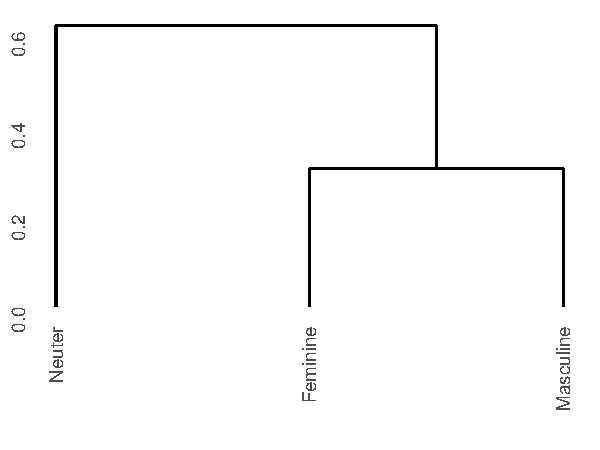
\includegraphics[scale=0.6]{./figures/latin/dendro-nouns.pdf}
    \subcaption{Clustering analysis on \tabref{tab:gender-lat-stats}.}
  \end{subfigure}%
  \begin{subfigure}{.5\textwidth}
    \centering
    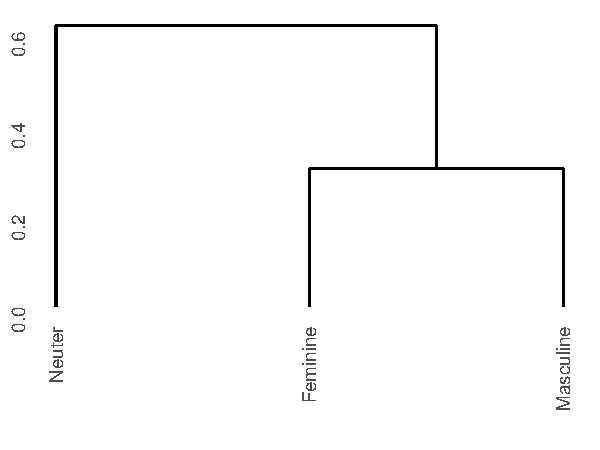
\includegraphics[scale=0.6]{./figures/latin/dendro-nouns-small.pdf}
    \subcaption{Clustering analysis on \tabref{tab:gender-lat-stats-2}.}
  \end{subfigure}
\caption{Clustering analysis for Latin gender assignment}\label{fig:clustering-latin}
\end{figure}

\is{hierarchical clustering}
\tabref{fig:clustering-latin} shows that the feminine and masculine nouns are closer to each other than they are to neuter nouns. This confirms the expectations of the \textsc{atc} model and matches the inflectional system where we find syncretism between the masculine and feminine.

\largerpage 
In conclusion, I have shown that in a very simple system like the one of Latin third declension nouns, the analogical model makes exactly the right predictions about how the three genders should cluster together based on formal properties of the \isi{stem}s. We see the same result for both datasets, with and without gender assigning suffixes.

\il{Latin|)}
\is{inflection!nominal|)}

\section{Gender vs inflection class: Romanian}

\subsection{The Romanian gender and plural system}

\il{Romanian|(}
\is{inflection!nominal|(}

A much more interesting gender and number system can be found in Romanian. Like Latin, Romanian is often analyzed as having three genders, which it inherited from Latin \autocite[23]{Gonczol.2007}. The interesting aspect of Romanian gender is that the neuter does not have a dedicated marker, but patterns with the masculine in the \isi{singular} and with the feminine in the plural. As Cojocaru explains, this phenomenon can be observed on all elements that agree with a noun. 

\begin{quotation}
The distinctive part of the neuter gender in Romanian is that it does not have any formal particularities. The neuter nouns in the singular look like masculine nouns, while in the plural they look like feminine nouns. The same applies to adjectives, pronouns and pronominal adjectives. When they modify or replace a neuter noun in the singular they appear in their masculine singular form, and when they modify or substitute a neuter noun in the plural they appear in their feminine plural form. \autocite[27]{Cojocaru.2003}
\end{quotation}

One striking example of this situation is illustrated by the three inflection classes in \tabref{tab:gender-rom}, each of which is found in only one gender. In this part of the system, neuter nouns inflect like masculine nouns in the \isi{singular}, and like feminine nouns in the plural. This means that, while there are no specific markers for neuter nouns, there is a three way split in the system.

\begin{table}
  \centering
  \begin{tabular}{llll}
    \lsptoprule
              & singular                   & plural                    & gloss           \\
    \midrule
    masculine & \cellcolor{gray!25}condr-u & condr-i                    & \textit{forest} \\
    neuter    & \cellcolor{gray!25}muze-u  & \cellcolor{gray!25}muze-e & \textit{museum} \\
    feminine  & cas-ă                      & \cellcolor{gray!25}cas-e  & \textit{house}  \\
    \lspbottomrule
  \end{tabular}
  \caption{Three way gender system in Romanian}\label{tab:gender-rom}
\end{table}

In terms of agreement, we see the same phenomenon (adapted from \citealt{Farkas.1990}), as can be observed in examples \REF{romanian-masc-exe}--\REF{romanian-neut-exe}:

\largerpage[2]
\begin{exe}
    \ex \label{romanian-masc-exe} masculine
    \begin{xlist}
        \ex 
        \gll Un trandafir alb e scump.\\
        a.\textsc{masc.sg} rose white.\textsc{masc.sg} is expensive.\textsc{masc.sg}\\
        \glt `A white rose is expensive.'
        \ex 
        \gll Unii.\textsc{masc.pl} trandafiri alb-\textit{i} sunt scump-\textit{i}.\\
        some rose white-\textsc{masc.pl} is expensive-\textsc{masc.pl}\\
        \glt `Some white roses are expensive.'
    \end{xlist}
    \end{exe}
%    \newpage
    
    \begin{exe}
    \ex feminine
    \begin{xlist}
        \ex 
        \gll O garoafa alb-\textit{a} e scump-\textit{a}.\\
        a.\textsc{fem.sg} carnation white-\textsc{fem.sg} is expensive-\textsc{fem.sg}\\
        \glt `A white carnation is expensive.'
        \ex 
        \gll Unele garoafe alb-\textit{e} sunt scump-\textit{e}.\\
        some.\textsc{fem.pl} carnation white-\textsc{fem.pl} is expensive-\textsc{fem.pl}\\
        \glt `Some white carnation are expensive.'
    \end{xlist}

    \ex \label{romanian-neut-exe} neuter
    \begin{xlist}
        \ex 
        \gll Un scaun alb e scump.\\
        a.\textsc{masc.sg} chair white.\textsc{masc.sg} is expensive.\textsc{masc.sg}\\
        \glt 'A white chair is expensive.'
        \ex 
        \gll Unele scaune alb-\textit{e} sunt scump-\textit{e}.\\
        some.\textsc{fem.pl} chairs white-\textsc{fem.pl} are expensive-\textsc{fem.pl}\\
        \glt `Some white chairs are expensive.'
    \end{xlist}
\end{exe}

\is{exception}
Here we have the identical type of distribution for agreement, as we saw for markers in \tabref{tab:gender-rom}. The word \textit{alb} `white' has the same marker (namely \textit{-ø}) when modifying a masculine or neuter noun in the singular, and it has the same marker (namely \textit{-e}) when modifying a neuter or feminine noun in the plural. So, even though there are only two different agreement markers in the plural and in the singular\footnote{In \REF{romanian-masc-exe} one could argue either that the consonant is the marker, or that there is a \textit{-$\emptyset$} marker.}, the alignment pattern produces three genders. Additionally, Romanian has a relatively complex inflection class system for singular and plural. \tabref{tab:romanian-plural-clases} presents the basic classes \autocite{Cojocaru.2003}\footnote{Classes \textit{iu--ie} and \textit{u--ă} in the neuter are classified as exceptions by the author.}. Usually, the singular is taken to be a sort of simplex form, instead of being composed of a stem and a singular marker. I take a slightly different approach here and consider the singular to be composed of a stem and a singular marker.

\begin{table}[!htbp]
  \centering
  \begin{tabular}{lllll}
    \lsptoprule
    Sg. marker & Pl. marker & Singular           & Plural             & Gloss            \\
        \midrule
    \multicolumn{5}{c}{Masculine nouns}                                                  \\
    \midrule
    -C         & -C+i       & elev      & elev\textit{i}     & `school student' \\
    -u         & -i         & le\textit{u}       & le\textit{i}       & `lion'           \\
    -e         & -i         & iepur\textit{e}    & iepur\textit{i}    & `rabbit'         \\
    -i         & -i         & och\textit{i}      & och\textit{i}      & `eye'            \\
    -ă         & -i         & tat\textit{ă}      & taț\textit{i}      & `father'         \\
    \midrule
    \multicolumn{5}{c}{Feminine nouns}                                                   \\
    \midrule
    -ă         & -e         & cas\textit{ă}      & cas\textit{e}      & `house'          \\
    -ă         & -i         & us\textit{ă}       & us\textit{i}       & `door'           \\
    -ă         & -uri       & marf\textit{ă}     & mărf\textit{uri}   & `merchandise'    \\
    -e         & -i         & lum\textit{e}      & lum\textit{i}      & `world'          \\
    -V+ie      & -V+i       & ba\textit{ie}      & bă\textit{i}       & `bathroom'       \\
    -C+ie      & -C+ii      & frecț\textit{ie}   & frecț\textit{ii}   & `massage'        \\
    -a         & -ale       & basm\textit{a}     & basm\textit{ale}   & `handkerchief'   \\
    -ea        & -ele       & caf\textit{ea}     & caf\textit{ele}    & `coffee'         \\
    -i         & -i         & marț\textit{i}     & marț\textit{i}     & `Tuesday'        \\
    \midrule
    \multicolumn{5}{c}{Neuter nouns}                                                     \\
    \midrule
    -C         & -C+uri     & tren      & tren\textit{uri}   & `train'          \\
    -C         & -C+e       & capac     & capac\textit{e}    & `lid'            \\
    -u         & -uri       & lucr\textit{u}     & lucr\textit{uri}   & `thing'          \\
    -u         & -e         & muze\textit{u}     & muze\textit{e}     & `museum'         \\
    -u         & -ă         & ou        & ou\textit{ă}       & `egg'            \\
    -iu /ju/   & -ii /ij/   & exerciț\textit{iu} & exerciț\textit{ii} & `exercise'       \\
    -iu /iw/   & -ie /i.e/  & sicr\textit{iu}    & sicr\textit{ie}    & `coffin'         \\
    -i  /j/    & -ie /je/   & tramva\textit{i}   & tramva\textit{ie}  & `tram'           \\
    -i  /i/    & -iuri      & tax\textit{i}      & tax\textit{iuri}   & `taxi'           \\
    -e         & -e         & num\textit{e}      & num\textit{e}      & `name'           \\
    \lspbottomrule
  \end{tabular}\caption{Number inflection classes in Romanian}\label{tab:romanian-plural-clases}
\end{table}

\tabref{tab:romanian-plural-clases} shows the problematic issue in the interaction between Romanian gender and number markers. Although gender correlates with inflection class, knowing the gender of a noun in Romanian is not enough for knowing its plural (or singular) form. Based on this fact, it has been argued that Romanian does not have three genders but rather a complex interaction between number markers. The most recent of these accounts is offered by \textcite{Bateman.2010}. The authors, partially following previous proposals by \textcite{Hall.1965} and \textcite{Farkas.1995}, claim that there are only two genders in Romanian, masculine and feminine, and that it is not gender that determines plural formation, but plural formation that helps determine gender in Romanian:
%
\nocite{Gerdts.2010} % just cite Gerdts book
\largerpage[2]
\begin{quotation}
Our position is supported by the fact that in traditional three-gender analyses there is limited predictability of plural endings for nouns in the same class, clearly showing that gender specification alone does not predict plural form \autocite[53]{Bateman.2010}
\end{quotation}

Similarly, they claim that a two-gender system for Romanian is more parsimonious than a three gender system because ``the same factors relevant for plural formation are indirectly relevant for predicting gender assignment and agreement in the plural'' \autocite[45]{Bateman.2010}.

To address the problem of agreement in Romanian nouns, \textcite[52]{Bateman.2010} propose that ``Romanian has two noun classes in the singular and in the plural'' but clarify that ``this categorization is not lexically specified''. These classes are in turn different for plural and singular. The first aspect of their system is easy to model with a type system, but the clarification that said noun classes are not lexically specified, less so. For this model, all lexemes in Romanian would be underspecified for a lexical class feature, which would only be specified after an inflectional process derives the singular or plural form of the noun.

For the \isi{singular}, \textcite{Bateman.2010} propose classes A and B. Traditionally feminine nouns belong to class A, while traditionally masculine and neuter nouns belong to class B. Class assignment in the singular is driven by both formal and semantic features (since animate nouns can straightforwardly be categorized as feminine or masculine, as well as other minor semantic classes). For the plural, the authors propose classes C and D. Class D includes traditional masculine nouns, while class C includes all other nouns. Again, class membership is determined by semantic and formal cues, where the formal cues are the plural endings of the nouns. A graphic representation of the two gender model is shown in \tabref{fig:graphic-two-gender-bateman}

\begin{figure}
    \caption{Two gender model for Romanian} \label{fig:graphic-two-gender-bateman}
    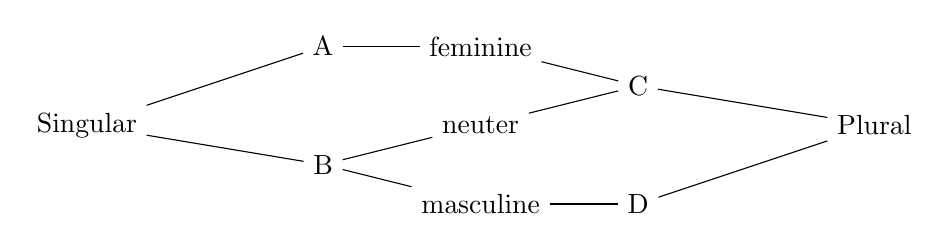
\begin{tikzpicture}[baseline=(current bounding box.north)]
        \node (Sg) at (0,0) {Singular};
        \node (A) at (3,1) {A};
        \node (B) at (3,-0.5) {B};
        \node (feminine) at (5,1) {feminine};
        \node (neuter) at (5,0) {neuter};
        \node (masculine) at (5,-1) {masculine};
        \node (C) at (7,0.5) {C};
        \node (D) at (7,-1) {D};
        \node (Pl) at (10,0) {Plural};
        \draw (Sg) -- (A);
        \draw (Sg) -- (B);
        \draw (A) -- (feminine);
        \draw (B) -- (neuter);
        \draw (B) -- (masculine);
        \draw (feminine) -- (C);
        \draw (neuter) -- (C);
        \draw (masculine) -- (D);
        \draw (C) -- (Pl);
        \draw (D) -- (Pl);
    \end{tikzpicture}
\end{figure}

\is{exception}
In the model by \textcite{Bateman.2010}, it is the plural class that determines gender:

\begin{quotation}
  In fact, with the exception of traditional masculines, all of which take the plural marker \textit{-i}, there are very few feminine and neuter nouns for which gender classification alone can predict plural form. For example, feminine nouns ending in \textit{-e} take the \textit{-i} plural marker [\dots]. As we mentioned previously, there are also feminine nouns ending in stressed \textit{-a} or \textit{-ea} that take the \textit{-le} plural marker, and there are neuter nouns ending in a stressed \textit{-ı} and borrowings from French ending in \textit{-ow} that take \textit{-uri} in the plural. Notice that in each of these cases the plural ending is determined by the noun’s ending rather than its gender class, which supports our claim that the plural forms determine class membership in the plural, rather than the other way around \autocite[54]{Bateman.2010}
\end{quotation}

This approach has recently received some support from a computational model. \textcite{Dinu.2012} present systems based on two support vector machines, one trained on plurals and one trained on \isi{singular}s, which manages to distinguish neuter nouns very well, at around 99\% accuracy (for two previous computational approaches see \citealt{Cucerzan.2003} and \citealt{Nastase.2009}). \textcite[123]{Dinu.2012} mention that their model supports Bateman and Polinsky's (2010) model, as plural class is in fact distinguishable for nouns from purely formal cues, and that gender is not needed. It is not completely clear from the study by \textcite{Dinu.2012} study, however, that gender would not provide extra information about plural formation. First, the authors looked at singular and plural words in the nominative, which means that their model had number information which is highly correlated with gender. A second issue is that the authors only considered the effect of formal cues for predicting gender, but did not fit a model that took into account the effect of gender.

Other solutions for modelling gender in Romanian have been proposed in different linguistic theories. Probably the most well known is \textcite{Farkas.1995}, who take an underspecification approach, where feminine nouns are specified as +\textsc{fem}, masculine nouns as -\textsc{fem}, and neuter nouns are not specified for gender (see also \citealt{Farkas.1990}, as well as \citealt{Sadler.2006, Wechsler.2008, Kramer.2015}). These approaches assume the existence of three genders, but diverge in how exactly their interrelations are implemented.

A different approach is pursued by \textcite{Steriade.2008}. \citeauthor{Steriade.2008} identifies some phonological \isi{constraint}s on the plural choice of some nouns. Her approach, however, focuses on the different phonological processes that \isi{stem}s undergo with certain markers, rather than on the actual choice of different markers. I will ignore stem processes in this study, but the approach developed in Chapter \ref{chap:complex} for Spanish could be extended to the Romanian system.

\is{inflection!nominal|)}

\subsection{Modelling the system}

The two gender model as presented by \textcite{Bateman.2010} has a conceptual problem. There are three types of nouns in Romanian based on their agreement behaviour. The discussion of how this originates and what features are responsible for this phenomenon is somewhat of a red herring. The fact is that we have three agreement patterns, and whether we need a lexically specified feature for this is a different question. Additionally, the argument that we do not need gender because inflection class is predictable from formal features, and because gender does not completely determine inflectional class, is not very convincing.

It is not really surprising that declension class is partially independent of gender, since this is not all that rare typologically speaking (\cite{Corbett.1991}, and Chapter \ref{chap:complex}), and it is even present in other Romance languages. A simple example is Spanish, where exponents of the singular only partially correlate with gender \autocite{Harris.1991}. Similarly, the fact that gender does not completely determine \isi{inflection class} does not entail that gender has no information about the inflection class of a noun, independently of other formal features on the noun. Incomplete information does not mean no information.

As for the Romanian system, what does make sense in the two-gender proposed by \textcite{Bateman.2010}, is to have four agreement classes, two for singular and two for plural, and many different actual inflection classes according to the singular-plural marker combination. This idea is depicted in the hierarchy \tabref{fig:romanian-hierar}.

\begin{figure}
    \caption{Romanian Gender-Number hierarchy} \label{fig:romanian-hierar}
    % \leavevmode\vadjust{\vspace{-\baselineskip}\newline
    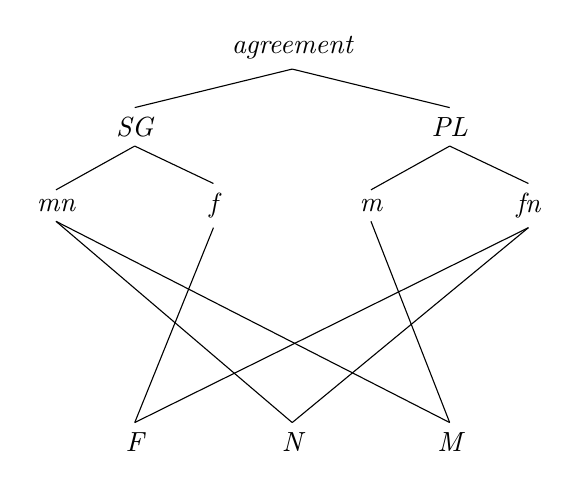
\begin{tikzpicture} [baseline=(current bounding box.north), every text node part/.style={align=center}]
        \node (top) at (1,4) {\it agreement};
        \node (SG) at (-1,3) {\it SG};
        \node (PL) at (3,3) {\it PL};
        \draw (top.south) -- (SG.north);
        \draw (top.south) -- (PL.north);
        \node (mn) at (-2,2) {\it mn};
        \node (f) at (0,2) {\it f};
        \draw (SG.south) -- (f.north);
        \draw (SG.south) -- (mn.north);
        \node (fn) at (4,2) {\it fn};
        \node (m) at (2,2) {\it m};
        \draw (PL.south) -- (fn.north);
        \draw (PL.south) -- (m.north);
        \node (F) at (-1,-1) {\it F};
        \node (N) at (1,-1) {\it N};
        \node (M) at (3,-1) {\it M};
        \draw (fn.south) -- (F.north);
        \draw (f.south) -- (F.north);
        \draw (m.south) -- (M.north);
        \draw (mn.south) -- (M.north);
        \draw (mn.south) -- (N.north);
        \draw (fn.south) -- (N.north);
        % \node (F1) at (-2,0) {\it u--i};
        % \node (F2) at (-1,0) {\it e--i};
        % \node (F3) at (0,0) {\it i--i};
    \end{tikzpicture}
\end{figure}

This hierarchy is exclusively about agreement because it indicates what the agreement would be with a given adjective. Notice that only listing the plural and singular for each noun is insufficient because adjectives do not agree with nouns in terms of markers, but in terms of gender as shown in \REF{romanian-exe-gender}.

%\newpage

\begin{exe}
    \ex \label{romanian-exe-gender}
    \begin{xlist}
        \ex 
        \gll tren-\textit{uri} mic-\textit{i}\\
        train.\textsc{masc.pl} small.\textsc{masc.pl}\\
        \glt `small trains'
        \ex 
        \gll lum-\textit{e} mic-\textit{ă}\\
        world.\textsc{fem.pl} small.\textsc{fem.pl}\\
        \glt `small world'
        \ex 
        \gll lucr-\textit{u} mic\\
        thing.\textsc{neut.pl} small.\textsc{neut.pl}\\
        \glt `small thing'
    \end{xlist}
\end{exe}

The adjective \textit{mic} `small' has three forms: \textit{mic} (masculine and neuter singular), \textit{mică} (feminine singular) and \textit{mici} (plural). This adjective does not agree with the number markers on the nouns, but with their gender.

Because, as we saw, gender does not completely determine \isi{inflection class}, this dimension needs to be modelled separately. For each gender, there are some markers, either singular or plural, which are unique to said gender. So, for example, the plural maker \textit{-iuri} is only found with neuter nouns, the singular marker \textit{-C+ie} only occurs with feminine nouns, and the plural marker \textit{-C+i} is only found with masculine nouns. This is crucial because we cannot claim that masculine and neuter nouns share all singular markers, or that feminine and neuter nouns share all plural markers. Markers like \textit{-ă} are found in the singular with feminine and masculine nouns, and in the plural with neuter nouns. Except for the classes where both the singular and plural use the same marker, markers are uniquely determined by the number they express. That is, even though the marker \textit{-ă} can express singular or plural, knowing the gender of the noun immediately resolves the uncertainty. In the case of \textit{-e} in feminine nouns, we need to know the other marker of the noun to be able to tell whether \textit{-e} is a plural or singular marker.


\begin{table}[p]
  \centering
  \begin{tabular}{lrrr}
    \lsptoprule
           & feminine & masculine & neuter \\
    \midrule
    a--ale  & 172      & 0         & 0      \\
    a--e    & 178      & 0         & 0      \\
    ă--e    & 11647    & 0         & 0      \\
    a--i    & 56       & 0         & 0      \\
    ă--i    & 2855     & 51        & 0      \\
    ă--uri  & 1590     & 0         & 0      \\
    C--e    & 0        & 0         & 7746   \\
    C--i    & 0        & 7252      & 0      \\
    C--ii   & 0        & 0         & 25     \\
    C--uri  & 0        & 0         & 5586   \\
    ea--ale & 1        & 0         & 0      \\
    ea--ele & 384      & 0         & 0      \\
    e--e    & 807      & 0         & 155    \\
    e--i    & 13814    & 227       & 0      \\
    e--iuri & 0        & 0         & 3      \\
    e--uri  & 17       & 0         & 90     \\
    i--e    & 0        & 0         & 31     \\
    ie--e   & 112      & 0         & 0      \\
    ie--ii  & 6771     & 0         & 0      \\
    ie--Vi  & 171      & 0         & 0      \\
    i--i    & 75       & 567       & 0      \\
    i--ie   & 0        & 0         & 189    \\
    i--iuri & 0        & 0         & 237    \\
    iu--ie  & 0        & 0         & 19     \\
    iu--ii  & 0        & 0         & 348    \\
    u--ă    & 0        & 0         & 1      \\
    u--e    & 0        & 0         & 936    \\
    u--i    & 0        & 700       & 0      \\
    u--uri  & 0        & 0         & 456    \\
    \lspbottomrule
  \end{tabular}
\caption{Number classes by gender in Romanian}\label{tab:decl-rom-gender}
\end{table}

\is{exception}
The issue becomes even clearer when we look at how the different number classes distribute across genders in \tabref{tab:decl-rom-gender} (see next section for an explanation of the dataset). What we clearly see here is that, with the exception of the classes\footnote{I use the notation \textit{sg--pl}.} \textit{ă--i}, \textit{e--e}, \textit{e--uri} and \textit{i--i}, declension class determines gender. We also see that the confusion is with the feminine, i.e. the masculine and neuter classes are never confused. Notice that this has the reverse structure of the agreement pattern, where neuter patterns with masculine and feminine, but these two do not pattern together.

\largerpage[2]
There are some additional classes not listed in \textcite{Cojocaru.2003}. For example, \textit{nutria} `otter' forms its plural as \textit{nutrii}. Similarly, \textit{anaconda} `anaconda' forms its plural as \textit{anaconde}. I leave these classes in as they are, but recognize that they might be special cases of foreign words or particular exceptions.\footnote{The markers \textit{-i} and \textit{-Vi} for the plural feminine could be collapsed into a single \textit{-i} marker. For consistency with \textcite{Cojocaru.2003}, I keep them as distinct markers, but in the end this decision should not really make much of a difference.}

The distribution of \isi{singular} and plural markers can be seen in \tabref{tab:sing-rom-gender} and \tabref{tab:plur-rom-gender}. In these distributions, we find something similar to what we had in the distribution of classes. Although there are markers that are shared by all three genders, namely \textit{-i} and \textit{-e} in the singular, there are no markers that are only shared by the neuter and feminine in the singular, and the only marker shared by the masculine and feminine is \textit{-ă}, with a suspiciously low type frequency in the masculine. On the other hand, in the plural, except for \textit{-i}, sharing of markers is only found between neuter and feminine.

With these facts in mind, there are three alternatives for a hierarchy of number markers in Romanian. If we wanted to keep the symmetry in the hierarchy between plural and \isi{singular}, we could separate the markers that cross `the wrong' classes into two. There are two potential justifications for this move, one theoretical and one empirical. Thinking in terms of simplicity, adding three additional singular markers, and one additional plural marker reduces the complexity of the hierarchy. The second reason has to do with the relative type frequencies of the problematic markers. If we look at their distributions, in the singular, \textit{-ă} and \textit{-e}, as shown in \tabref{tab:sing-rom-gender}, are \textit{much} more common with the feminine than with the masculine or neuter. In a similar way, \textit{-i} has more or less the same type frequency for the neuter and masculine, and it is less frequent with the feminine. In the plural, \textit{-i} is much more frequent with the feminine than the masculine.

\begin{table}
  \centering
  \begin{tabular}{lrrr}
    \lsptoprule
    & Feminine & Masculine & Neuter \\
    \midrule
    a  & 406     & 0        & 0      \\
    ă  & 16092   & 51       & 0      \\
    C  & 0       & 7252     & 13357  \\
    e  & 14638   & 227      & 248    \\
    ea & 385     & 0        & 0      \\
    i  & 75      & 567      & 457    \\
    ie & 7054    & 0        & 0      \\
    iu & 0       & 0        & 367    \\
    u  & 0       & 700      & 1393   \\
    \lspbottomrule
  \end{tabular}
  \caption{Singular classes by gender in Romanian}\label{tab:sing-rom-gender}
\end{table}

\begin{table}
  \centering
  \begin{tabular}{lrrr}
    \lsptoprule
    & Feminine & Masculine & Neuter \\
    \midrule
    ă    & 0       & 0        & 1      \\
    ale  & 173     & 0        & 0      \\
    e    & 12744   & 0        & 8868   \\
    ele  & 384     & 0        & 0      \\
    i    & 16800   & 8797     & 0      \\
    ie   & 0       & 0        & 208    \\
    ii   & 6771    & 0        & 373    \\
    iuri & 0       & 0        & 240    \\
    uri  & 1607    & 0        & 6132   \\
    Vi   & 171     & 0        & 0      \\
    \lspbottomrule
  \end{tabular}
  \caption{Plural classes by gender in Romanian}\label{tab:plur-rom-gender}
\end{table}

Pursuing a symmetric approach, the system would have \textit{-e}$_{f}$, \textit{-i}$_{f}$, \textit{-ă}$_{f}$ and \textit{-e}$_{mn}$, \textit{-i}$_{mn}$ and \textit{-ă}$_{m}$ in the singular; and \textit{-i}$_{m}$ and \textit{-i}$_{nf}$ in the plural. In  \figref{fig:romanian-hierar-markers} we see what a hierarchy under these assumptions would look like.


%\clearpage 

\begin{figure}
    \caption{Romanian marker hierarchy} \label{fig:romanian-hierar-markers}
    % \leavevmode\vadjust{\vspace{-\baselineskip}\newline
    \resizebox{0.9\textwidth}{!}{%
      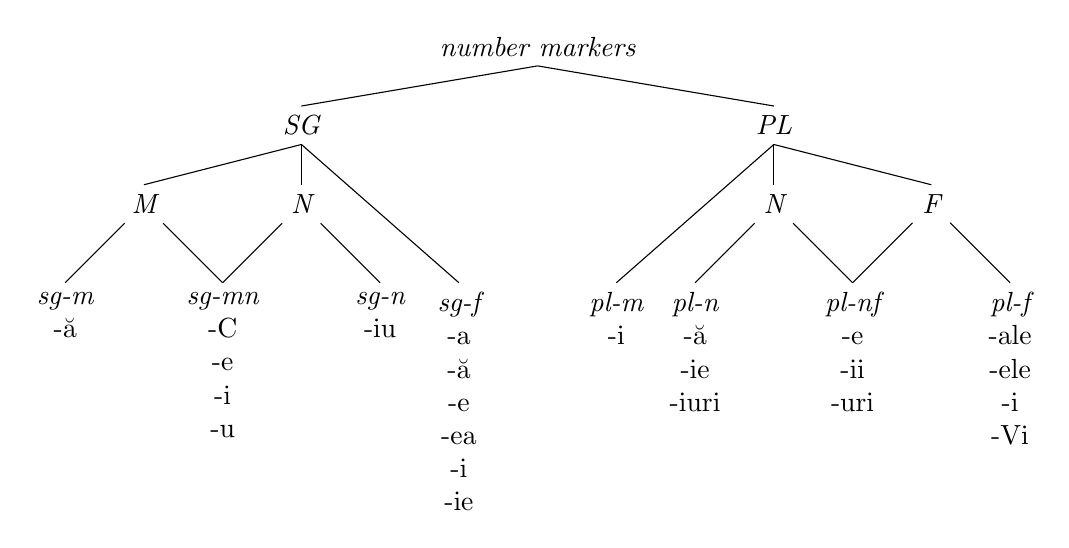
\begin{tikzpicture} [baseline=(current bounding box.north), every text node part/.style={align=center}]
        \tikzset{
          m2style/.style={style={nodes={text width=3.5em,anchor=center}},
          },
        }
        \node (top) at (7,4) {\it number markers};
        \node (SG) at (4,3) {\it SG};
        \node (PL) at (10,3) {\it PL};
        \draw (top.south) -- (SG.north);
        \draw (top.south) -- (PL.north);
        \node (msg) at (2,2) {\it M};
        \node (nsg) at (4,2) {\it N};
        \node [anchor=north](fsg) at (6,1) {\it sg-f \\ -a \\ -ă \\ -e \\ -ea \\ -i \\ -ie};
        \draw (SG.south) -- (fsg.north);
        \draw (SG.south) -- (msg.north);
        \draw (SG.south) -- (nsg.north);
        \node [anchor=north](mpl) at (8,1) {\it pl-m \\ -i};
        \node (npl) at (10,2) {\it N};
        \node (fpl) at (12,2) {\it F};
        \draw (PL.south) -- (fpl.north);
        \draw (PL.south) -- (mpl.north);
        \draw (PL.south) -- (npl.north);
        \node [anchor=north](sgm) at (1,1) {\it sg-m \\ -ă};
        \node [anchor=north](sgmn) at (3,1) {\it sg-mn \\ -C \\ -e \\ -i \\ -u};
        \node [anchor=north](sgn) at (5,1) {\it sg-n \\ -iu};
        % 
        \node [anchor=north](pln) at (9,1) {\it pl-n \\ -ă \\ -ie \\ -iuri};
        \node [anchor=north](plnf) at (11,1) {\it pl-nf \\ -e \\ -ii \\ -uri};
        \node [anchor=north](plf) at (13,1) {\it pl-f \\ -ale \\ -ele \\ -i \\ -Vi};
        % 
        \draw (pln.north) -- (npl);
        \draw (plnf.north) -- (npl);
        \draw (plnf.north) -- (fpl);
        \draw (plf.north) -- (fpl);
        % 
        \draw (sgm.north) -- (msg);
        \draw (sgmn.north) -- (nsg);
        \draw (sgmn.north) -- (msg);
        \draw (sgn.north) -- (nsg);
    \end{tikzpicture}}
\end{figure}

An alternative is to have an asymmetric hierarchy, but fewer individual markers. A sketch of this hierarchy can be seen in \tabref{fig:romanian-hierar-markers-2}. In this case, there is no real symmetry between the singular and the plural, nor is there any with the agreement patterns.

\begin{figure}
    \caption{Symmetric Romanian marker hierarchy} \label{fig:romanian-hierar-markers-2}
    % \leavevmode\vadjust{\vspace{-\baselineskip}\newline
    \resizebox{0.9\textwidth}{!}{%
      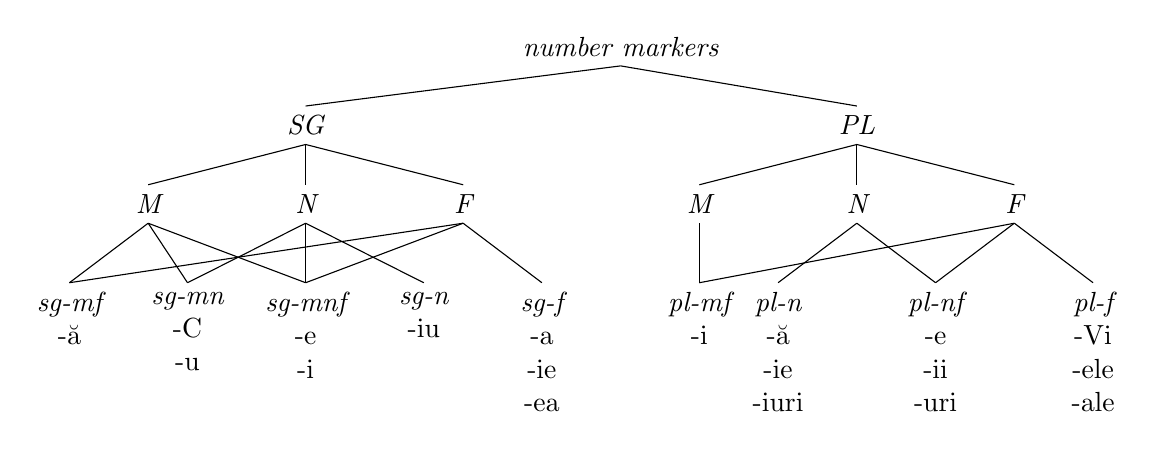
\begin{tikzpicture} [baseline=(current bounding box.north), every text node part/.style={align=center}]
        \tikzset{
          m2style/.style={style={nodes={text width=3.5em,anchor=center}},
          },
        }
        \node (top) at (8,4) {\it number markers};
        \node (SG) at (4,3) {\it SG};
        \node (PL) at (11,3) {\it PL};
        \draw (top.south) -- (SG.north);
        \draw (top.south) -- (PL.north);
        \node (Msg) at (2,2) {\it M};
        \node (Nsg) at (4,2) {\it N};
        \node (Fsg) at (6,2) {\it F};
        \draw (SG.south) -- (Fsg.north);
        \draw (SG.south) -- (Msg.north);
        \draw (SG.south) -- (Nsg.north);
        \node (Mpl) at (9,2) {\it  M};
        \node (Npl) at (11,2) {\it N};
        \node (Fpl) at (13,2) {\it F};
        \draw (PL.south) -- (Fpl.north);
        \draw (PL.south) -- (Mpl.north);
        \draw (PL.south) -- (Npl.north);
        % 
        \node [anchor=north](msg) at (1,1) {\it sg-mf \\ -ă};
        \node [anchor=north](mnsg) at (2.5,1) {\it sg-mn \\ -C \\ -u};
        \node [anchor=north](mnfsg) at (4,1) {\it sg-mnf \\ -e \\ -i};
        \node [anchor=north](fsg) at (7,1) {\it sg-f \\ -a \\ -ie \\ -ea};
        \node [anchor=north](nsg) at (5.5,1) {\it sg-n \\ -iu};
        \draw (Msg.south) -- (msg.north);
        \draw (Fsg.south) -- (msg.north);
        \draw (Msg.south) -- (mnsg.north);
        \draw (Nsg.south) -- (mnsg.north);
        \draw (Nsg.south) -- (nsg.north);
        \draw (Fsg.south) -- (mnfsg.north);
        \draw (Msg.south) -- (mnfsg.north);
        \draw (Nsg.south) -- (mnfsg.north);
        \draw (Fsg.south) -- (fsg.north);
        % 
        \node [anchor=north](mfpl) at (9,1) {\it pl-mf \\ -i};
        \node [anchor=north](npl) at (10,1) {\it pl-n \\ -ă \\ -ie\\-iuri};
        \node [anchor=north](nfpl) at (12,1) {\it pl-nf \\ -e \\ -ii \\ -uri};
        \node [anchor=north](fpl) at (14,1) {\it pl-f \\ -Vi \\ -ele \\ -ale};
        \draw (Mpl.south) -- (mfpl.north);
        \draw (Fpl.south) -- (mfpl.north);
        \draw (Fpl.south) -- (fpl.north);
        \draw (Fpl.south) -- (nfpl.north);
        \draw (Npl.south) -- (npl.north);
        \draw (Npl.south) -- (nfpl.north);
    \end{tikzpicture}}
\end{figure}

The final inflection classes result from specifying pairings between the \isi{singular} and plural markers shown in \tabref{tab:romanian-plural-clases}. Since there is no free combination between singular and plural markers, each class must be specified directly.

\largerpage 
The third alternative consists of two independent flat lists for \isi{singular} and plural markers and then specify each \isi{inflection class} as in \tabref{fig:romanian-hierar-markers-2}. A simplified hiearchy for this approach is given in \tabref{fig:romanian-hierar-markers-3}. The advantage of this model is that it is simpler than the previous two, in that it requires less complex interactions between types. The downside is that the partial correlations between gender and inflection class would be lost.

\begin{figure}
    \caption{Simplified Romanian marker hierarchy} \label{fig:romanian-hierar-markers-3}
    % \leavevmode\vadjust{\vspace{-\baselineskip}\newline
    \resizebox{0.9\textwidth}{!}{%
      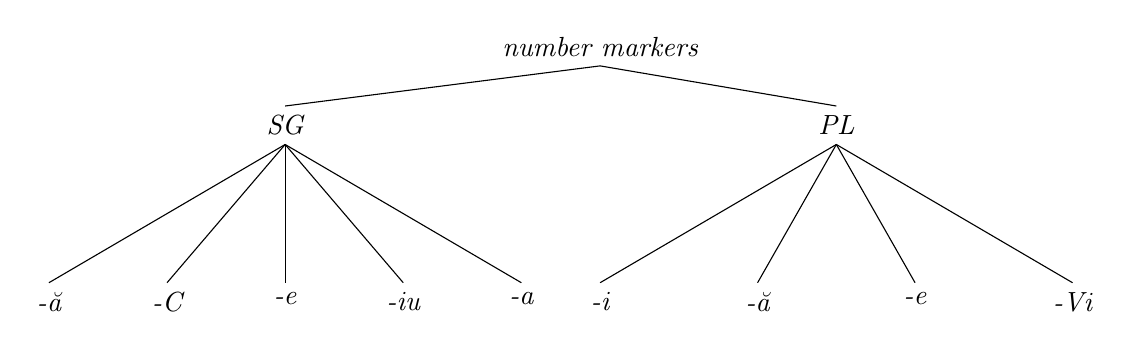
\begin{tikzpicture} [baseline=(current bounding box.north), every text node part/.style={align=center}]
        \tikzset{
          m2style/.style={style={nodes={text width=3.5em,anchor=center}},
          },
        }
        \node (top) at (8,4) {\it number markers};
        \node (SG) at (4,3) {\it SG};
        \node (PL) at (11,3) {\it PL};
        \draw (top.south) -- (SG.north);
        \draw (top.south) -- (PL.north);
        % 
        \node [anchor=north](msg) at (1,1) {\it -ă};%;
        \node [anchor=north](mnsg) at (2.5,1) {\it -C};% \\ -u};
        \node [anchor=north](mnfsg) at (4,1) {\it -e};% \\ -i};
        \node [anchor=north](fsg) at (7,1) {\it -a};% \\ -ie \\ -ea};
        \node [anchor=north](nsg) at (5.5,1) {\it -iu};%;
        \draw (SG.south) -- (msg.north);
        \draw (SG.south) -- (mnsg.north);
        \draw (SG.south) -- (nsg.north);
        \draw (SG.south) -- (mnfsg.north);
        \draw (SG.south) -- (fsg.north);
        % 
        \node [anchor=north](mfpl) at (8,1) {\it  -i};
        \node [anchor=north](npl) at (10,1) {\it  -ă};%\\ -ie\\-iuri};
        \node [anchor=north](nfpl) at (12,1) {\it  -e};% \\ -ii \\ -uri};
        \node [anchor=north](fpl) at (14,1) {\it  -Vi};% \\ -ele \\ -ale};
        \draw (PL.south) -- (mfpl.north);
        \draw (PL.south) -- (fpl.north);
        \draw (PL.south) -- (npl.north);
        \draw (PL.south) -- (nfpl.north);
    \end{tikzpicture}}
\end{figure}

There is no way of deciding apriori which of these three approaches is better. The choice between the three will depend on considerations pertaining to what a theory of morphology should look like. They do, however, make slightly different predictions in terms of what we should find in the analogical model. In the first hierarchy, we would expect there to be little to no confusion between feminine, masculine and neuter nouns, and there should be a separation between the classes with the \textit{-e}, \textit{-ă} and \textit{-i} markers in the \isi{singular}, as well as those with the \textit{-i} markers in the plural. That is, these dimensions should not be available for the analogical model.

The hierarchy in \tabref{fig:romanian-hierar-markers-2} predicts that those three markers should be available for nouns to cluster together, and we should thus see classes clustering around these markers. Similarly, these classes should allow for some limited confusion between masculine and feminine, especially in the classes with the shared markers.

\is{hierarchical clustering}
Finally, the hierarchy in \tabref{fig:romanian-hierar-markers-3} predicts that clustering should be exclusively about markers and not around gender. Therefore, we would expect classes with shared markers to cluster together, but not classes forming clusters around the genders they correlate with. The hierarchies in \tabref{fig:romanian-hierar-markers} and \tabref{fig:romanian-hierar-markers-2} do predict some clustering around genders and some clustering around markers.

\subsection{Data}

For this study, I used the Romanian dictionary DEX Online (https://dexonline.ro), taking the data base from the python api \autocite{Navalici.2013}. From the dictionary\footnote{More specifically, from the \texttt{dex\_lexemes}, \texttt{dex\_lexems\_inflections} and \texttt{dex\_inflections} data bases provided. The search targeted entries with the fields: \textit{plural}, \textit{nearticulat}, \textit{Substantive} and \textit{Nominative}.}, I extracted all nouns in the nominative form for which a plural form was specified. From these, I removed all nouns with a plural form ending in \textit{s} because these are clear borrowings from Spanish and other languages. Finally, I removed all nouns with common gender. This process gives us 63646 nouns. For each noun, I extracted the plural and singular markers according to the description in \textcite{Cojocaru.2003} and added the extra classes not listed there.

The distribution of nouns by gender in the extracted corpus is, for a total of 63501 nouns: 38737 feminine nouns, 8891 masculine nouns and 15873 neuter nouns.

\subsubsection{Methodology and hypothesis}

There are basically two claims at stake. On the one hand, it has been argued that gender information is not helpful when figuring out the plural form of nouns in Romanian. On the other hand, we want to test which of the three \isi{inflection class} configurations makes more accurate predictions regarding the analogical relations between the \isi{stem}s of the nouns.

To test the first claim, we can fit two different analogical models: (i) one that only looks at phonological information, which would approximate proposals for gender assignment based on the ending of nouns in Romanian like those of \textcite{Vrabie.1989} and \textcite{Vrabie.2000}; (ii) and then a similar model that also looks at gender information. If gender carries no useful information about the plural form of nouns in Romanian, as \textcite{Bateman.2010} claim, then we should see no difference in the performance of each of the models. If adding gender clearly increases accuracy, we can say that there is a high probability that gender does in fact play a role in predicting inflection class\footnote{We cannot have complete certainty because it is always possible that a different model solely based on formal cues could outperform the model including gender.}.

To test the second claim, we can look at the overall gender+inflection class distribution. For this second part, I used a reduced and more balanced dataset. For each noun, I extracted its class as a tuple: \textit{gender}+\textit{singular}+\textit{plural}. This produces a total of 57 classes, 17 feminines, 14  masculines and 26 neuters. The distribution of classes by type frequency can be seen in \tabref{fig:rumanian-classes}. From these, I removed the three lowest frequency classes (marked in red in \tabref{fig:rumanian-classes}), and took a random sample of up to 3000 nouns for the more frequent classes. This produces a somewhat more balanced dataset.

\begin{figure}
  \centering
  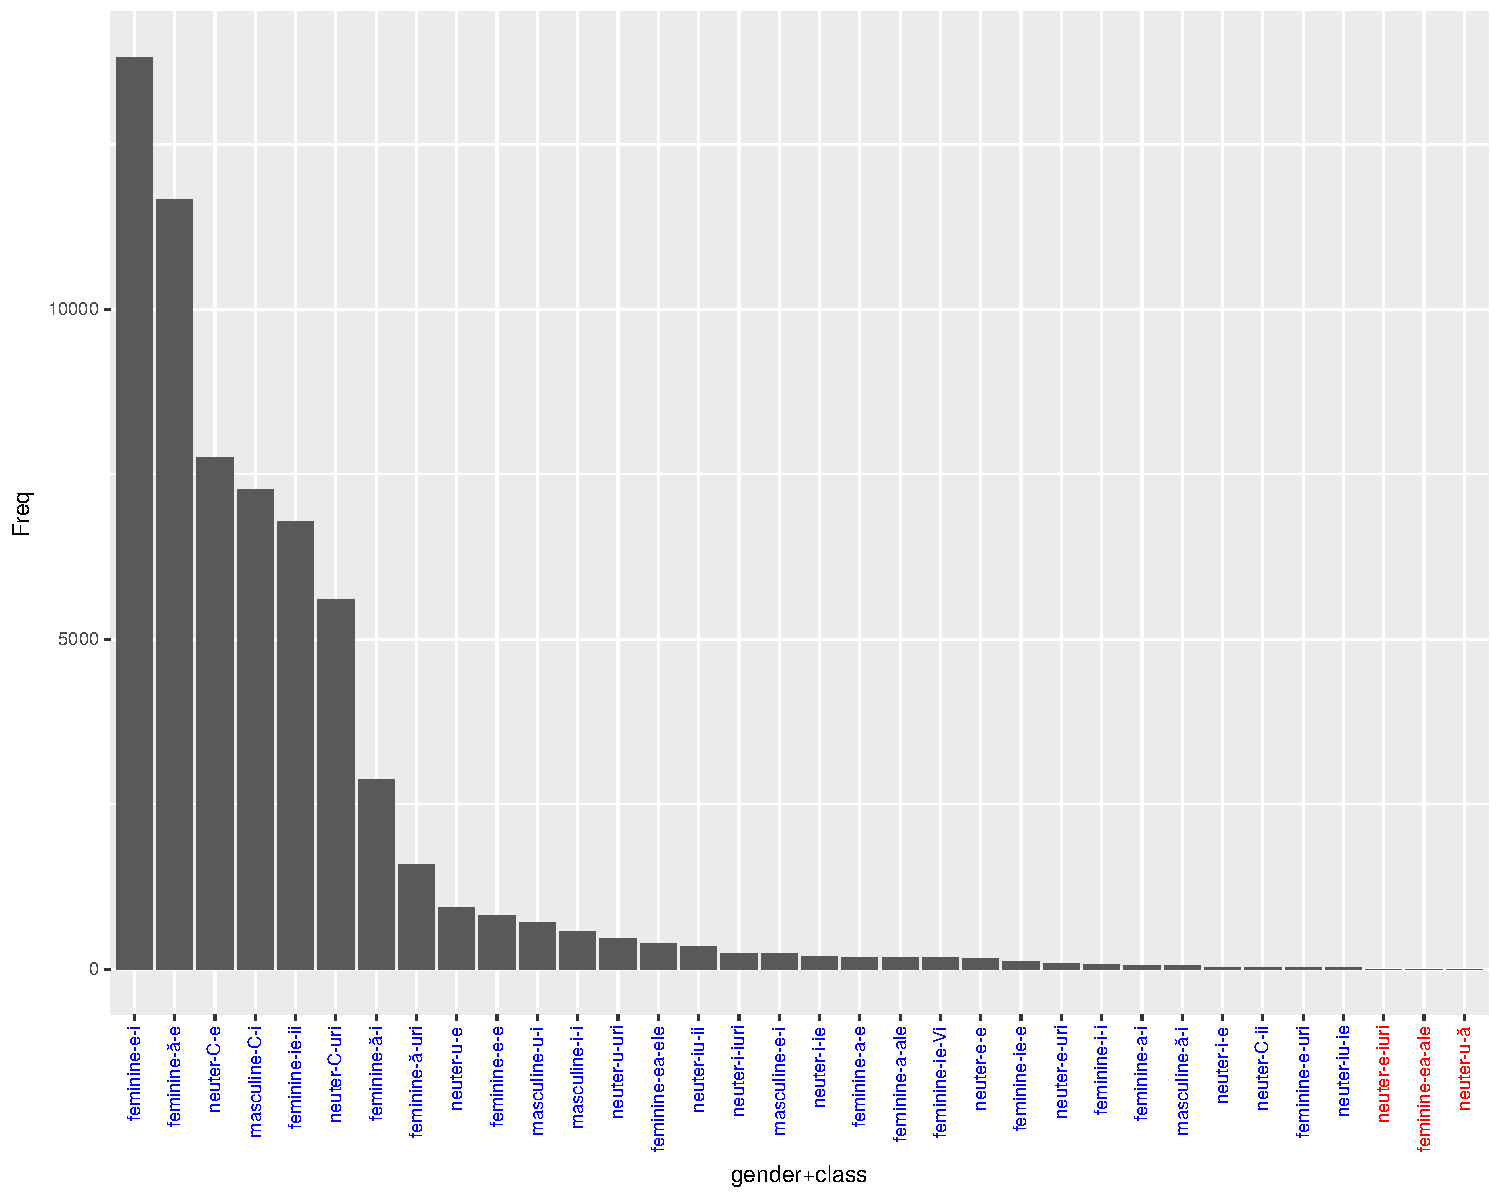
\includegraphics[width=0.9\textwidth]{./figures/romanian/nclasses-plot.pdf}
  \caption{Class frequency}\label{fig:rumanian-classes}
\end{figure}

The basic prediction is that neuter classes should be confused with feminine and masculine classes, but these two should not be confused with each other.

\subsection{Results}

\subsubsection{Predicting gender}

First, we predict gender from the shape of the \isi{stem}s with the formula: \texttt{gender $\sim$ final.1 + final.2 + final.3 + n\_vowels}.\footnote{There were no hidden nodes and a decay rate of 0.} Here we are simply looking at the final three segments and the number of vowels in the stem. The results can be seen in \tabref{tab:gender-romanian} and \tabref{tab:gender-romanian-stats}. The tables show that gender is in fact predictable without any information about number markers. However, in \tabref{tab:gender-romanian} we do see that there is a relatively large confusion between masculine and neuter, and between neuter and feminine, but not so much between feminine and masculine. This is again confirmed in \tabref{tab:gender-romanian-distance} (larger numbers mean more distance between the classes). This observation matches the hierarchy in \tabref{fig:romanian-hierar}, where feminine and masculine genders do not share any set of common nodes, but masculine and neuter, and feminine and neuter do.

\begin{table}
  \centering
  \begin{tabular}{rrrr}
    \lsptoprule
    \multicolumn{4}{c}{Reference}              \\
    \midrule
    Prediction & Feminine & Masculine & Neuter \\
    Feminine   & 14314    & 783       & 1750   \\
    Masculine  & 80       & 665       & 494    \\
    Neuter     & 987      & 2926      & 6246   \\
    \lspbottomrule
  \end{tabular}
  \caption{Confusion Matrix for the model predicting Gender of Romanian nouns}\label{tab:gender-romanian}
\end{table}

\begin{table}[p]
  \centering
  \begin{tabular}{llrr}
    \lsptoprule
    \multicolumn{4}{c}{Overall statistics:} \\

    \midrule
    \multicolumn{4}{c}{Accuracy : 0.7515}                                  \\
    \multicolumn{4}{c}{95\% CI : (0.7464, 0.7565)}                         \\
    \multicolumn{4}{c}{No Information Rate : 0.5446}                       \\
    \multicolumn{4}{c}{Kappa : 0.5564}                                     \\
    \midrule
    \multicolumn{4}{c}{Statistics by Class:}                               \\
    \midrule
                      & Feminine & Masculine & Neuter \\
    Sensitivity       & 0.9306          & 0.1520           & 0.7357        \\
    Specificity       & 0.8031          & 0.9759           & 0.8019        \\
    Neg Pred Value    & 0.9064          & 0.8626           & 0.8759        \\
    Balanced Accuracy & 0.8669          & 0.5639           & 0.768         \\
    \lspbottomrule
  \end{tabular}
  \caption{Overall statistics for the Confusion Matrix in \tabref{tab:gender-romanian}}\label{tab:gender-romanian-stats}
\end{table}

\begin{table}
  \centering
  \begin{tabular}{rrrr}
    \lsptoprule
              & Feminine & Masculine \\
    \midrule
    Masculine & 2.346527 &           \\
    Neuter    & 2.256934 & 0.154508  \\
    \lspbottomrule
  \end{tabular}
  \caption{Distance matrix for the Confusion Matrix in \tabref{tab:gender-romanian}}\label{tab:gender-romanian-distance}
\end{table}

\subsubsection{Predicting singular}

Next, we turn to the number markers. In this case, we have several dimensions that need to be predicted. On the one hand, there are individual number markers, and on the other hand there are complete \isi{inflection class}es with and without gender distinctions. Because there are some inflection classes which can appear with two genders, it is interesting to ask how well we can distinguish these cases.  Additionally, because we are mostly interested in seeing how the clusters work, we can compare whether predicting inflection class without gender produces similar clusters to those we get when predicting inflection class with gender.

We start with the \isi{singular} markers with the formula: \texttt{singular $\sim$ final.1 + final.2 + final.3 + n\_vowels}\footnote{The model had no hidden nodes and a decay rate of 0.}. The results are given in \tabref{tab:singular-romanian} and \tabref{tab:singular-romanian-stats}. We see that the singular marker, as defined here, is relatively predictable, but not perfectly.

\begin{table}
  \centering
  \begin{tabular}{lrrrrrrrrr}
    \lsptoprule
    \multicolumn{10}{c}{Reference}                                         \\
    \midrule
    Prediction & a   & ă    & C    & e    & ea  & i   & ie   & iu  & u    \\
    a          & 15  & 17   & 15   & 3    & 5   & 2   & 7    & 0   & 2    \\
    ă          & 156 & 6181 & 361  & 813  & 205 & 315 & 677  & 156 & 37   \\
    C          & 117 & 232  & 8104 & 159  & 37  & 530 & 441  & 24  & 648  \\
    e          & 51  & 604  & 218  & 2993 & 25  & 63  & 186  & 68  & 25   \\
    ea         & 0   & 10   & 1    & 1    & 6   & 3   & 17   & 4   & 0    \\
    i          & 2   & 25   & 20   & 12   & 13  & 80  & 37   & 3   & 2    \\
    ie         & 45  & 379  & 181  & 72   & 76  & 87  & 1784 & 94  & 5    \\
    iu         & 1   & 9    & 0    & 2    & 7   & 1   & 6    & 12  & 3    \\
    u          & 19  & 54   & 126  & 16   & 10  & 19  & 128  & 6   & 1375 \\
    \lspbottomrule
  \end{tabular}
  \caption{Confusion Matrix for the model predicting the singular marker of Romanian nouns}\label{tab:singular-romanian}
\end{table}

\begin{table}[p]
  \centering
  \begin{tabular}{c}
    \lsptoprule
    Overall statistics: \\
    \midrule
    Accuracy : 0.7276                                 \\
    95\% CI : (0.7223, 0.7327)                        \\
    No Information Rate : 0.3196                      \\
    Kappa : 0.6425                                    \\
    \lspbottomrule
  \end{tabular}
  \caption{Overall statistics for the Confusion Matrix in \tabref{tab:singular-romanian}}\label{tab:singular-romanian-stats}
\end{table}

\subsubsection{Predicting plural}

\begin{table}[p]
  \centering
  \begin{tabular}{lrrrrrrrrr}
    \lsptoprule
    \multicolumn{10}{c}{Reference}                                      \\
    \midrule
    Prediction & ale & e    & ele & i    & ie & ii   & iuri & uri  & Vi \\
    ale        & 17  & 12   & 5   & 13   & 0  & 7    & 1    & 21   & 0  \\
    e          & 36  & 4570 & 106 & 1876 & 57 & 780  & 35   & 1053 & 56 \\
    ele        & 3   & 6    & 8   & 10   & 1  & 15   & 4    & 2    & 0  \\
    i          & 86  & 2415 & 121 & 7392 & 85 & 471  & 102  & 1219 & 61 \\
    ie         & 0   & 6    & 0   & 6    & 6  & 0    & 0    & 10   & 0  \\
    ii         & 25  & 530  & 85  & 187  & 3  & 1961 & 30   & 150  & 0  \\
    iuri       & 0   & 6    & 4   & 18   & 1  & 23   & 21   & 3    & 0  \\
    uri        & 5   & 665  & 55  & 796  & 55 & 117  & 43   & 2689 & 38 \\
    Vi         & 0   & 9    & 0   & 22   & 1  & 0    & 1    & 12   & 16 \\
    \lspbottomrule
  \end{tabular}
  \caption{Confusion Matrix for the model predicting the plural marker of Romanian nouns}
  \label{tab:plural-romanian}
\end{table}

\begin{table}[p]
  \centering
  \begin{tabular}{c}
    \lsptoprule
    Overall statistics: \\
    \midrule
    Accuracy : 0.5905\\
    95\% CI : (0.5848, 0.5963)\\
    No Information Rate : 0.3654\\
    Kappa : 0.4278\\
    \lspbottomrule
  \end{tabular}
  \caption{Overall statistics for the confusion matrix in \tabref{tab:plural-romanian}}\label{tab:plural-romanian-stats}
\end{table}

We now turn to plural markers. The model used is the same as for \isi{singular} markers, with the formula: \texttt{plural $\sim$ final.1 + final.2 + final.3 + n\_vowels}. The results for predicting plural markers are shown in \tabref{tab:plural-romanian} and \tabref{tab:plural-romanian-stats}. What we find is that the model can predict plural markers somewhat less accurately than singular markers. Nevertheless, the accuracy and kappa scores are quite far above random chance.



Now we address the claims by \textcite{Bateman.2010} that gender does not really help to determine the plural marker a noun will take, and that plural class assignment is solely based on phonological features (including the singular marker). Properly testing this claim is not possible because the authors do not provide a full model for plural assignment. However, one can compare a model that only includes phonological features (and the singular marker) to one which also includes gender.\footnote{Of course, there is always the possibility that a better model, solely based on phonological features, would outperform the model presented here.} We fit a model with the formula: \texttt{plural $\sim$ final.1 + final.2 + final.3 + n\_vowels + singular + gender}. The results can be seen in \tabref{tab:plural-romanian-2} below.

\begin{table}
  \centering
  \begin{tabular}{lrrrrrrrrr}
    \lsptoprule
    \multicolumn{10}{c}{Reference}                                        \\
    \midrule
    Prediction & ale & e    & ele & i    & ie  & ii   & iuri & uri  & Vi  \\
    ale        & 126 & 51   & 1   & 4    & 0   & 0    & 0    & 0    & 0   \\
    e          & 41  & 6308 & 0   & 473  & 0   & 21   & 16   & 1334 & 25  \\
    ele        & 0   & 0    & 383 & 0    & 0   & 0    & 0    & 0    & 0   \\
    i          & 5   & 712  & 0   & 9807 & 0   & 0    & 0    & 30   & 0   \\
    ie         & 0   & 0    & 0   & 0    & 170 & 9    & 42   & 0    & 0   \\
    ii         & 0   & 3    & 0   & 0    & 11  & 3333 & 0    & 5    & 4   \\
    iuri       & 0   & 13   & 0   & 0    & 28  & 1    & 179  & 0    & 0   \\
    uri        & 0   & 1093 & 0   & 36   & 0   & 9    & 0    & 3790 & 0   \\
    Vi         & 0   & 39   & 0   & 0    & 0   & 1    & 0    & 0    & 142 \\
    \lspbottomrule
  \end{tabular}
  \caption{Confusion Matrix for the model predicting the plural marker of Rumanian nouns with additional gender information}
  \label{tab:plural-romanian-2}
\end{table}

\begin{table}
  \centering
  \begin{tabular}{c}
    \lsptoprule
    Overall statistics: \\
    \midrule
    Accuracy : 0.8581\\
    95\% CI : (0.854, 0.8622)\\
    No Information Rate : 0.3654\\
    Kappa : 0.8063\\
    \lspbottomrule
  \end{tabular}
  \caption{Overall statistics for the confusion matrix in \tabref{tab:plural-romanian-2}}\label{tab:plural-romanian-stats-2}
\end{table}

Predicting the plural marker with all predictors (gender and \isi{singular} marker) gives us the results presented in \tabref{tab:plural-romanian-2}, and the corresponding statistics in \tabref{tab:plural-romanian-stats-2}. The model evaluation is given in \tabref{fig:romanian-eval-pl}. \tabref{fig:romanian-eval-pl} shows that removing gender from the model causes a very steep drop in accuracy, i.e. gender does help in the analogical model. These results clearly speak against \citeauthor{Bateman.2010}' (2010) claim that gender does not help distinguish plural classes. If this result is correct, then there are no strong arguments for a two gender system for Romanian.

\begin{figure}
  \centering
  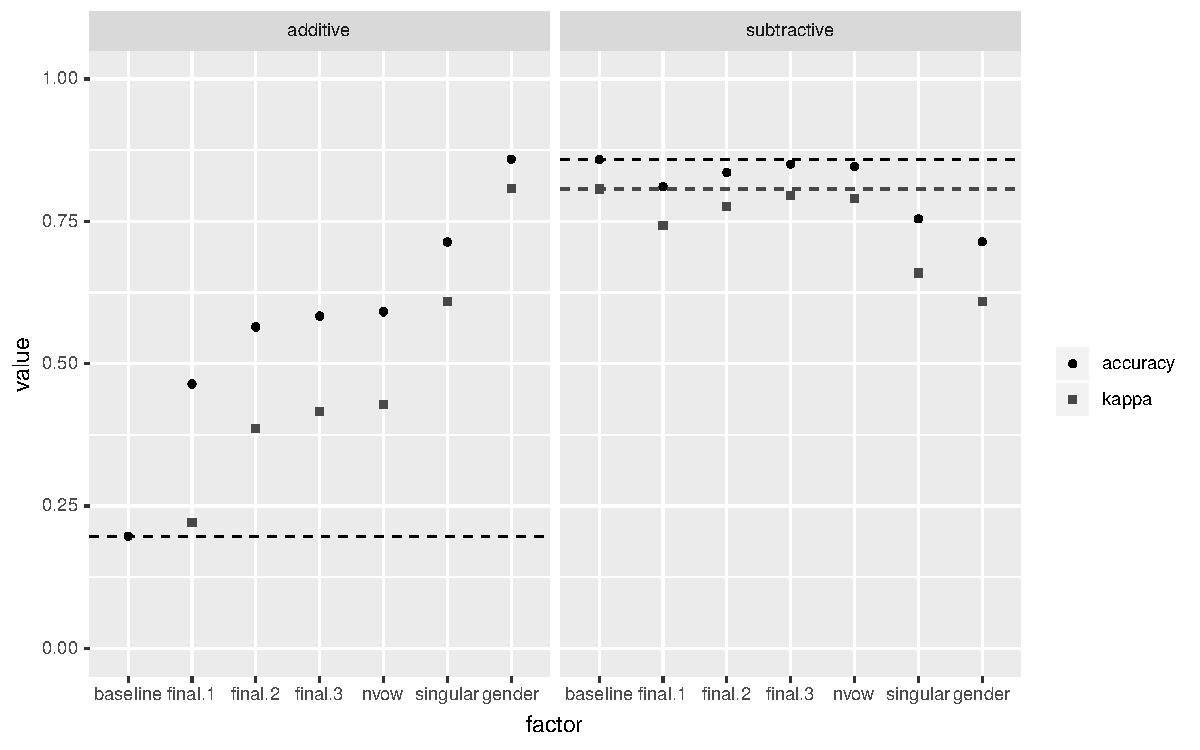
\includegraphics[width=1.0\textwidth]{./figures/romanian/plural-overall.pdf}
  \caption{Additive (left) and subtractive (right) accuracy and kappa scores for the model predicting plural in Romanian}\label{fig:romanian-eval-pl}
\end{figure}

\subsubsection{Inflection class}

\is{inflection!nominal|(}
Finally, we turn to the prediction of inflection class. Again, there are two possibilities we want to look at. First, we predict inflection class without making gender distinctions, i.e. if class \textit{e--e} is found in feminine and neuter, we assume this is a single class and not two different classes. We use the formula as before: \texttt{class $\sim$ final.1 + final.2 + final.3 + n\_vowels}. The results of this model can be seen in \tabref{fig:class-1-cm-romanian} and the corresponding statistics in \tabref{tab:class-1-romanian-stats}.

\begin{figure}
  \centering
  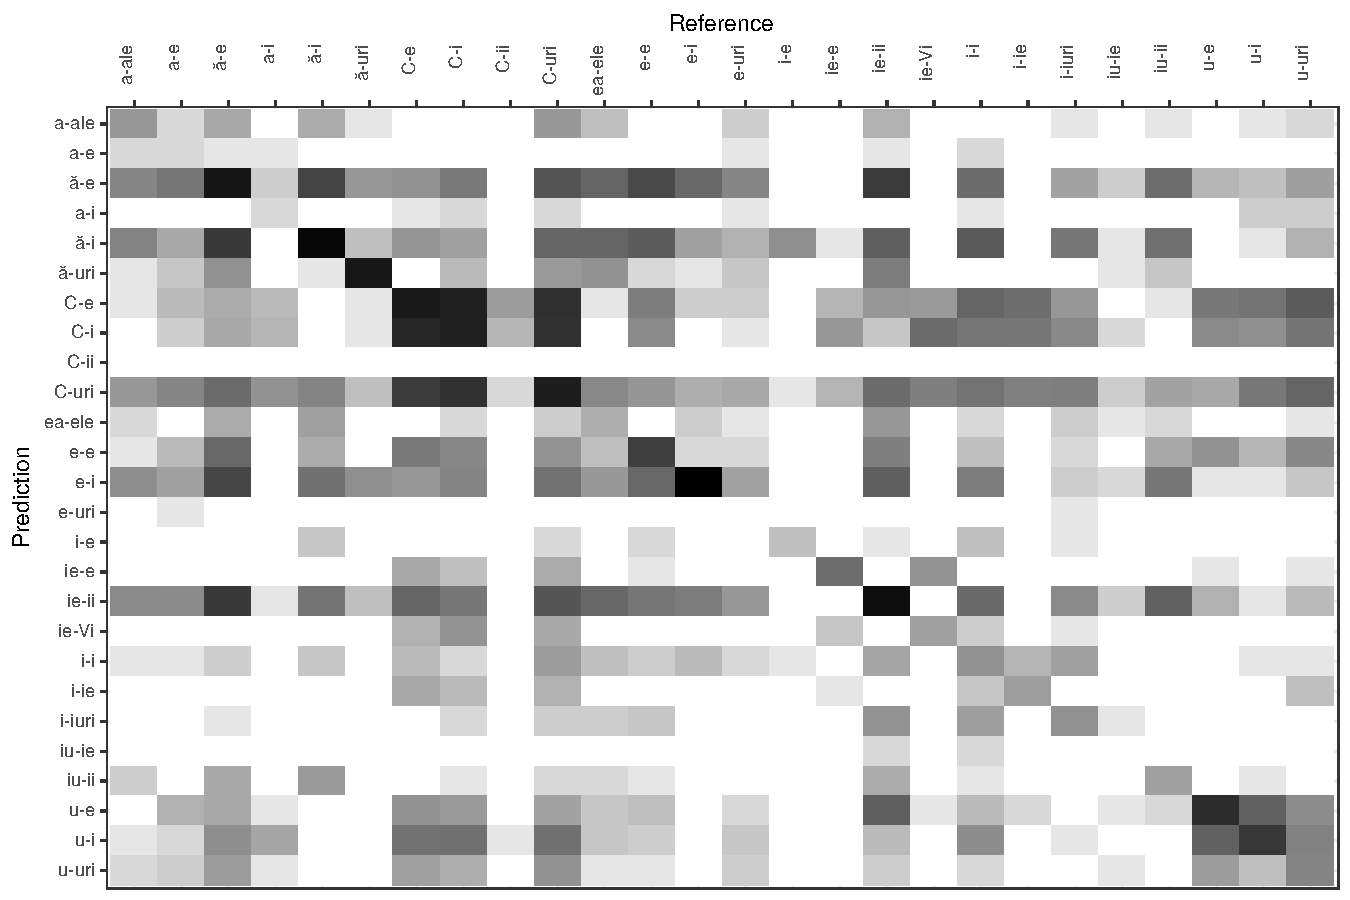
\includegraphics[width=1.0\textwidth]{./figures/romanian/class-1-cm.pdf}
  \caption{Heat map for the model predicting inflection class in Romanian}\label{fig:class-1-cm-romanian}
\end{figure}


\begin{table}
  \centering
  \begin{tabular}{c}
    \lsptoprule
    Overall statistics: \\
    \midrule
    Accuracy : 0.5577\\
    95\% CI : (0.5518, 0.5635)\\
    No Information Rate : 0.1062\\
    Kappa : 0.5121\\
    \lspbottomrule
  \end{tabular}
  \caption{Overall statistics for the heat map in \tabref{fig:class-1-cm-romanian}}\label{tab:class-1-romanian-stats}
\end{table}

\is{hierarchical clustering}
\tabref{tab:class-1-romanian-stats} shows that the model performs worse than the model predicting singular, but better (according to kappa score) than the model predicting only plurals. From the heat map in \tabref{fig:class-1-cm-romanian} it is clear that there is a high degree of confusion between the different classes, but it also looks like this confusion is not entirely random. The two strongest clusters of confusion are between classes with a \textit{-C} singular marker, and between classes with a \textit{-u} singular marker. If we perform cluster analysis on the corresponding similarity model, we get the results in \tabref{fig:romanian-clust-class-1}. In this figure, I have additionally indicated the gender information for the inflection class for convenience, but the model itself had no information about gender. What can be seen from the clustering is that, although there is organization along marker lines, the strongest clustering effect is that of gender. Additionally, whenever masculine classes cluster together with neuter classes, these share the same singular marker, and masculine only classes seem to only cluster with neuter classes.

\begin{figure}
  \centering
  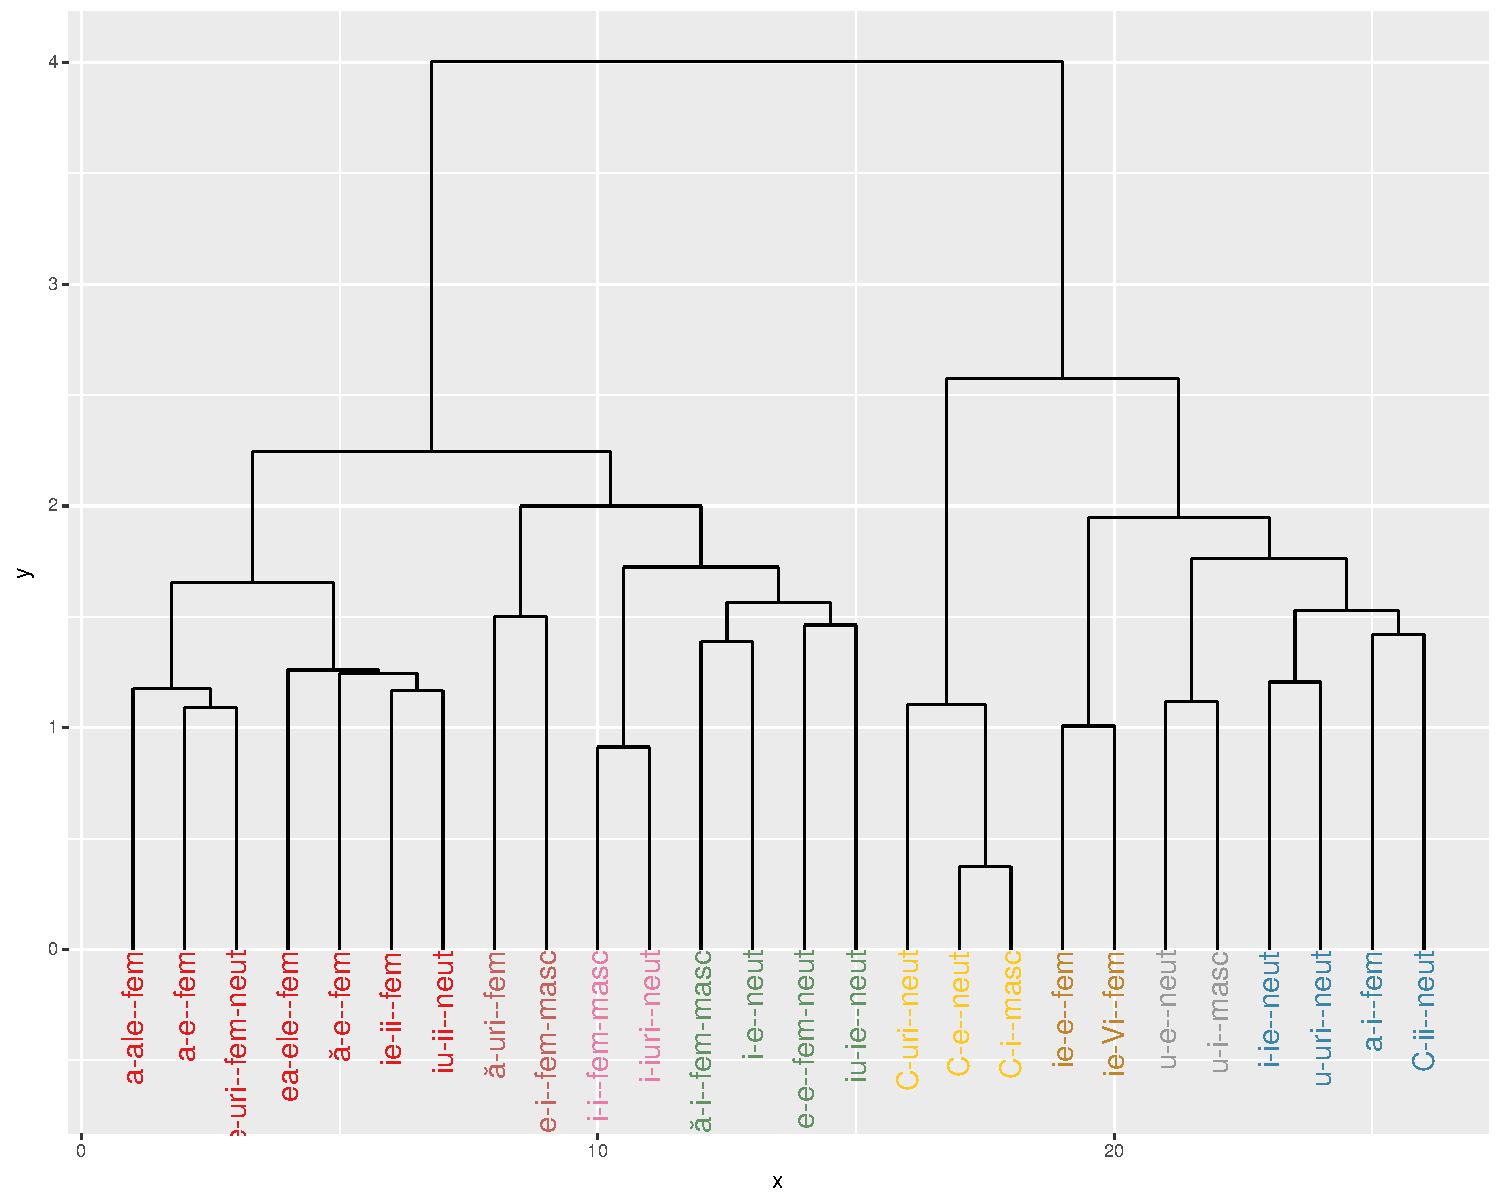
\includegraphics[width=0.9\textwidth]{./figures/romanian/romanian-clust-class-1.pdf}
  \caption{Clustering analysis of singular-plural class in Romanian}\label{fig:romanian-clust-class-1}
\end{figure}

Next, inflection classes are divided by gender, so that the five classes in the dataset which are ambiguous for gender are split into individual classes (one for each gender). For this model, the results are presented in \tabref{fig:class-2-cm-romanian} and the corresponding statistics in \tabref{tab:class-2-romanian-stats}. There is practically no difference in accuracy between both models. The clustering for this model is shown in \tabref{fig:romanian-clust-class-2}. This clustering reflects almost exactly the hierarchy in \tabref{fig:romanian-hierar-markers-2} on page \pageref{fig:romanian-hierar-markers-2}. Most clusters are found within a single same gender exclusively (clusters in light brown, light yellow, blue and dark gray), feminine and neuter, or masculine and neuter. Particularly clear are clusters where neuter and masculine share the same singular marker (clusters in pink, dark brown and light grey), or the feminine and neuter share the same plural marker (the cluster in green).  The only cluster including the three genders has the classes with singular markers \textit{-e} and \textit{-ă}. Marker \textit{-e} is the only one connected to all three genders in \tabref{fig:romanian-hierar-markers-2}, while \textit{-ă} is the only marker shared by feminine and masculine genders.

\begin{figure}
  \centering
  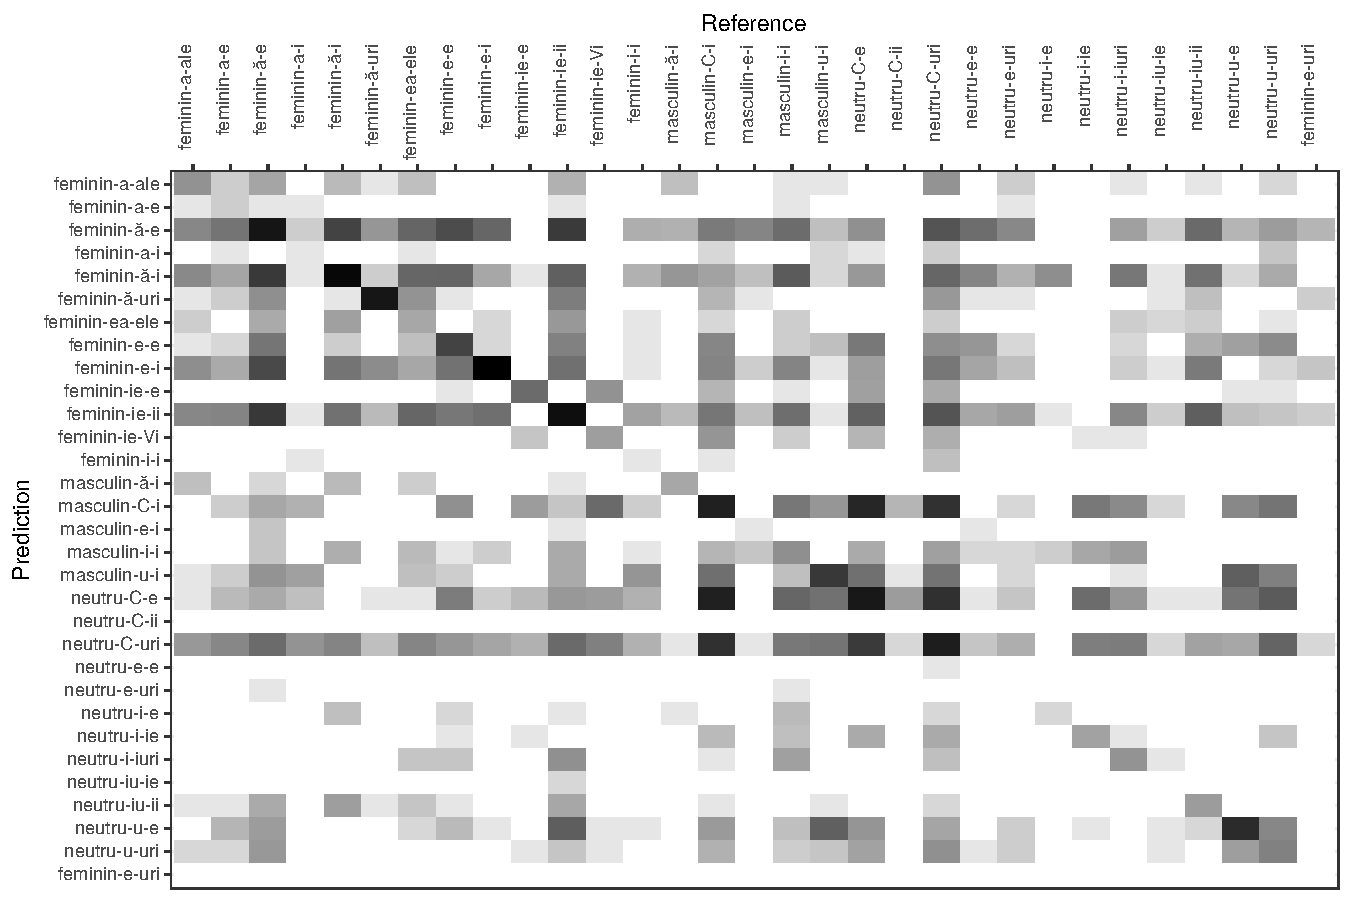
\includegraphics[width=1.0\textwidth]{./figures/romanian/class-2-cm.pdf}
  \caption{Heat map for the model predicting inflection class by gender in Romanian}\label{fig:class-2-cm-romanian}
\end{figure}

\begin{table}
  \centering
  \begin{tabular}{c}
    \lsptoprule
    Overall statistics: \\
    \midrule
    Accuracy : 0.5546\\
    95\% CI : (0.5488, 0.5605)\\
    No Information Rate : 0.1062\\
    Kappa : 0.5092\\
    \lspbottomrule
  \end{tabular}
  \caption{Overall statistics for the heat map in \tabref{fig:class-2-cm-romanian}}\label{tab:class-2-romanian-stats}
\end{table}

\begin{figure}
  \centering
  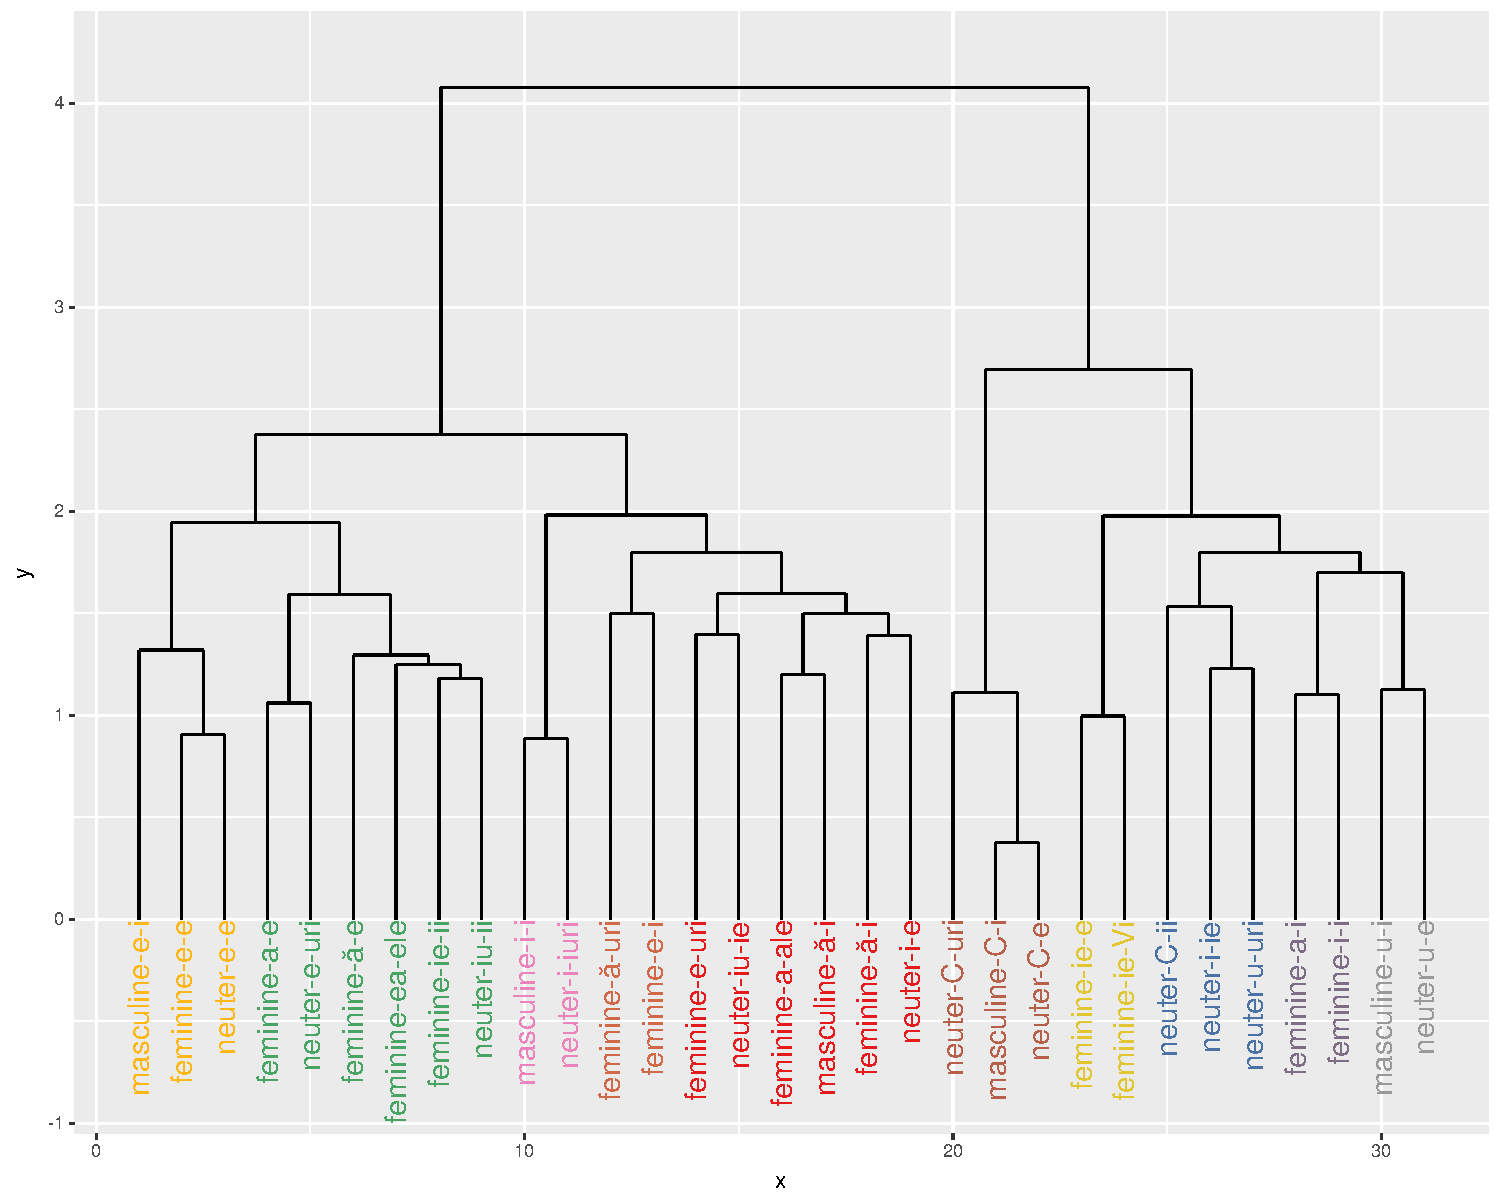
\includegraphics[width=0.9\textwidth]{./figures/romanian/romanian-clust.pdf}
  \caption{Clustering analysis of gender and class in Romanian}\label{fig:romanian-clust-class-2}
\end{figure}

\is{hierarchical clustering}
Romanian plural markers are strongly predictable from phonological features of nouns. The models presented here are a strong computational validation of \textcite{Vrabie.1989} and \textcite{Vrabie.2000}. The model by \textcite{Bateman.2010} is also partially supported in the sense that we see strong evidence for four agreement classes. But the model presented in this section also refutes \citeauthor{Bateman.2010} in that there is evidence for a gender-number interaction. More precisely, there is evidence that inflection classes are partially dependent on gender, and that gender is predictive of plural, even when phonological features are considered. Most importantly, we do not see any evidence for a flat inflection class hierarchy, nor for the more symmetric hierarchy in \tabref{fig:romanian-hierar-markers} or the simpler hierarchy in \tabref{fig:romanian-hierar-markers-3}, but we do see evidence for the hierarchy in \tabref{fig:romanian-hierar-markers-2}, where inflection classes are partially conditioned by their gender alignment.

\is{inflection!nominal|)}
\il{Romanian|)}

\section{Interim conclusion}

In this chapter I have presented two cases of gender-inflection class interactions, namely nouns from the Latin third declension and Romanian nouns. In Latin, we saw a relatively simple system where syncretisms in the inflection of nouns are conditioned by their gender. The Latin case could be modeled with a very simple tree clearly reflected in the analogical system. The nouns in Romanian presented a much more complex interaction between gender and inflection class. Therefore, a much more elaborate hierarchy had to be postulated. Still, I showed that the analogical model was helpful in distinguishing between the three alternatives.

With regards to the overall question of this book, in both cases we clearly saw that there are reflexes of the hierarchical structure in the analogical relations between the different classes.
\is{gender|)}
\is{inflection!nominal|)}

%%% Local Variables:
%%% mode: latex
%%% TeX-master: "../main"
%%% End:
